\section{Evaluation}
\label{sec:eval}
\vspace{10pt}

~\bu{Suggestions for creating a first draft:
\begin{itemize}
\item In Section 4.1: When describing our experimental setup, refer to Table 1 to say we restrict our attention to these 6 VMs from AWS and only use num cores, memory, num replicas, and throughput as our independent variables. Our dependent variables are average read and write latencies.
\item Have a generic figure showing a YCSB client and one of our case studies with 3 replicas. 
\item For Sections 4.2-4.4, describe the graphs/tables being presented in some detail, identify any trends. Conclude each with a list of "Key insights"
\item Most figures and tables need more clarity on what exactly was the training set, for which VM the prediction is being done, etc. All figures need larger fonts on their axes, labels, etc. 
\item Replace R-squared with $R^2_{predicted}$. 
\end{itemize}
    }

\subsection{Methodology and Setup}
\vspace{10pt}

\begin{table}
\centering

\begin{tabular}{|r|l|c|r|l|} \hline
Instance name & Abbr.& \# cores&Memory&Network\\ \hline
r3.large & $VM_1$ & 2 & 15 GB & Moderate\\ \hline
r3.xlarge & $VM_2$ & 4 & 30.5 GB & Moderate\\ \hline
r3.2xlarge & $VM_3$ & 8 & 61 GB & High\\ \hline
m3.large & $VM_4$ & 2 & 7.5 GB & Moderate\\ \hline
2m3.xlarge & $VM_5$ & 4 & 15 GB & Moderate\\ \hline
m3.2xlarge & $VM_6$ & 8 & 30 GB & High\\ \hline
\hline\end{tabular}
\caption{AWS instance types employed in our evaluation. }
\label{table:awstypes}
\end{table}

\mm{
We benchmarked virtual machines on the most widely used cloud vendor, Amazon Web Services (AWS).  We studied three different types of databases: Apache Cassandra (NoSQL database), Redis (Key-Value caching database), and MySQL (SQL database).

For benchmarking we used the open-source Yahoo! Cloud Serving Benchmark (YCSB).  For each test case we loaded the database with 1,000,000 records, each containing ten fields of 100 bytes each (the default).  YCSB defines several standard workloads; we used Workload B (95\% read 5\% write).  The requests for records were made using the zipfian probability distribution.

We ran the YCSB client on a m4.2xlarge EC2 instance running Ubuntu Linux 14.04. We monitored the system load average on the client machine to verify that the client was not the bottleneck during the tests.

Amazon EC2 is hosted in multiple geographic regions around the world, and multiple zones within each region.  The testing client and servers were all created within the same region (us-west) and availability zone (2b) to minimize the effect of network latency.

  \begin{figure}
  \centering
    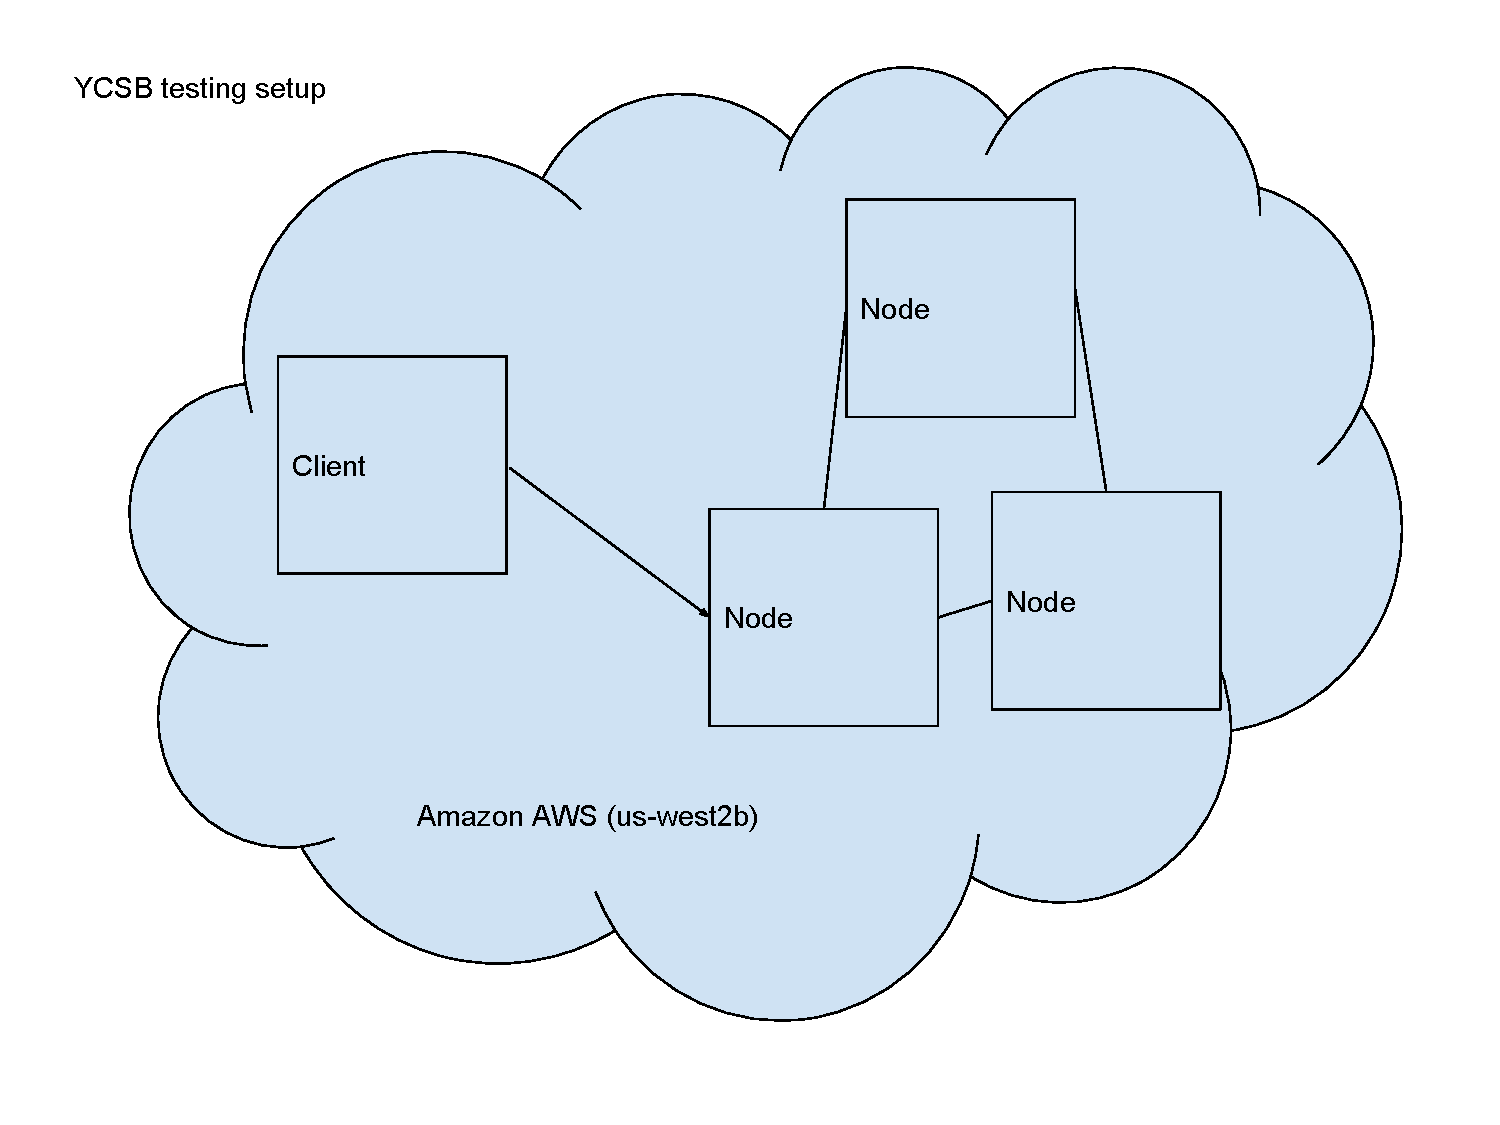
\includegraphics[scale = 0.25]{ycsb_diagram.pdf}
    \caption{YCSB benchmark TODO: PLACEHOLDER NEEDS IMPROVEMENT}
    \label{figure:ycsb}
  \end{figure}

}%

\subsection{Case Study 1: Redis}
\vspace{10pt}

\mm{
Redis is an open-source, key/value NoSQL database.  Redis is in-memory, and therefore very fast.  Redis also optionally supports persistence, so unlike memcached it can be used as a primary database or as a cache.

Redis was deployed on AWS using Amazon ElastiCache, a web service that abstracts the deployment and administration of the OS and database software.  Elasticache supports up to five read replicas of the primary database.  For our testing we only used a single read replica.

Using $VM_2$ for test data, we did a multiple linear regression on the training set for sizes 1 through 5 for the average read latency.  Each time another instance was added to the training set, the $R^2_{predicted}$ increased (Table \ref{table:redis}).  This was shown for multiple training sets, as show in Figure \ref{figure:redisbarread}.

The improving linear fit is visually demonstrated by the sequence of linear predicted values in Figure \ref{figure:redisfitread}.  The measured test values are denoted as circles, and the sequence of predicted values are shown as lines calculated from the values predicted by the sequence of linear regressions for larger training sets.

For the average write latency, the results were similar, as shown in Figure \ref{figure:redisbarwrite}.  The improving fit for write latency is shown in Figure \ref{figure:redisfitwrite}.

   }

\begin{table}
\centering
\caption{Redis $R_{predicted}^2$ for $VM_2$}
\begin{tabular}{|r|r|l|} \hline
$R_{read}^2$&$R_{write}^2$&Training Data\\ \hline
-0.648416 & -1.12245 & VM6 \\ \hline 
0.51488 & 0.547705 & VM6 VM5 \\ \hline 
0.738979 & 0.738969 & VM6 VM5 VM3 \\ \hline 
0.832156 & 0.821984 & VM6 VM5 VM3 VM1 \\ \hline 
0.837957 & 0.827944 & VM6 VM5 VM3 VM1 VM4 \\ \hline 
\hline\end{tabular}
\label{table:redis}
%\end{table}

%\begin{table}
\centering
\caption{Redis $R_{predicted}^2$ for $VM_2$}
\begin{tabular}{|r|r|l|} \hline
$R_{read}^2$&$R_{write}^2$&Training Data\\ \hline
-0.648416 & -1.12245 & VM6 \\ \hline 
0.506158 & 0.41527 & VM6 VM3 \\ \hline 
0.738979 & 0.738969 & VM6 VM3 VM5 \\ \hline 
0.776002 & 0.756578 & VM6 VM3 VM5 VM4 \\ \hline 
0.837957 & 0.827944 & VM6 VM3 VM5 VM4 VM1 \\ \hline 
\hline\end{tabular}
\label{table:redis}
%\end{table}

%\begin{table}
\centering
\caption{Redis $R_{predicted}^2$ for $VM_2$}
\begin{tabular}{|r|r|l|} \hline
$R_{read}^2$&$R_{write}^2$&Training Data\\ \hline
-0.559516 & -0.47657 & VM5 \\ \hline 
0.51488 & 0.547705 & VM5 VM6 \\ \hline 
0.738979 & 0.738969 & VM5 VM6 VM3 \\ \hline 
0.776002 & 0.756578 & VM5 VM6 VM3 VM4 \\ \hline 
0.837957 & 0.827944 & VM5 VM6 VM3 VM4 VM1 \\ \hline 
\hline\end{tabular}
\label{table:redis}
%\end{table}

%\begin{table}
\centering
\caption{Redis $R_{predicted}^2$ for $VM_2$}
\begin{tabular}{|r|r|l|} \hline
$R_{read}^2$&$R_{write}^2$&Training Data\\ \hline
-0.559516 & -0.47657 & VM5 \\ \hline 
0.260701 & 0.29636 & VM5 VM3 \\ \hline 
0.738979 & 0.738969 & VM5 VM3 VM6 \\ \hline 
0.776002 & 0.756578 & VM5 VM3 VM6 VM4 \\ \hline 
0.837957 & 0.827944 & VM5 VM3 VM6 VM4 VM1 \\ \hline 
\hline\end{tabular}
\label{table:redis}
\end{table}

  \begin{figure}
    \centering
    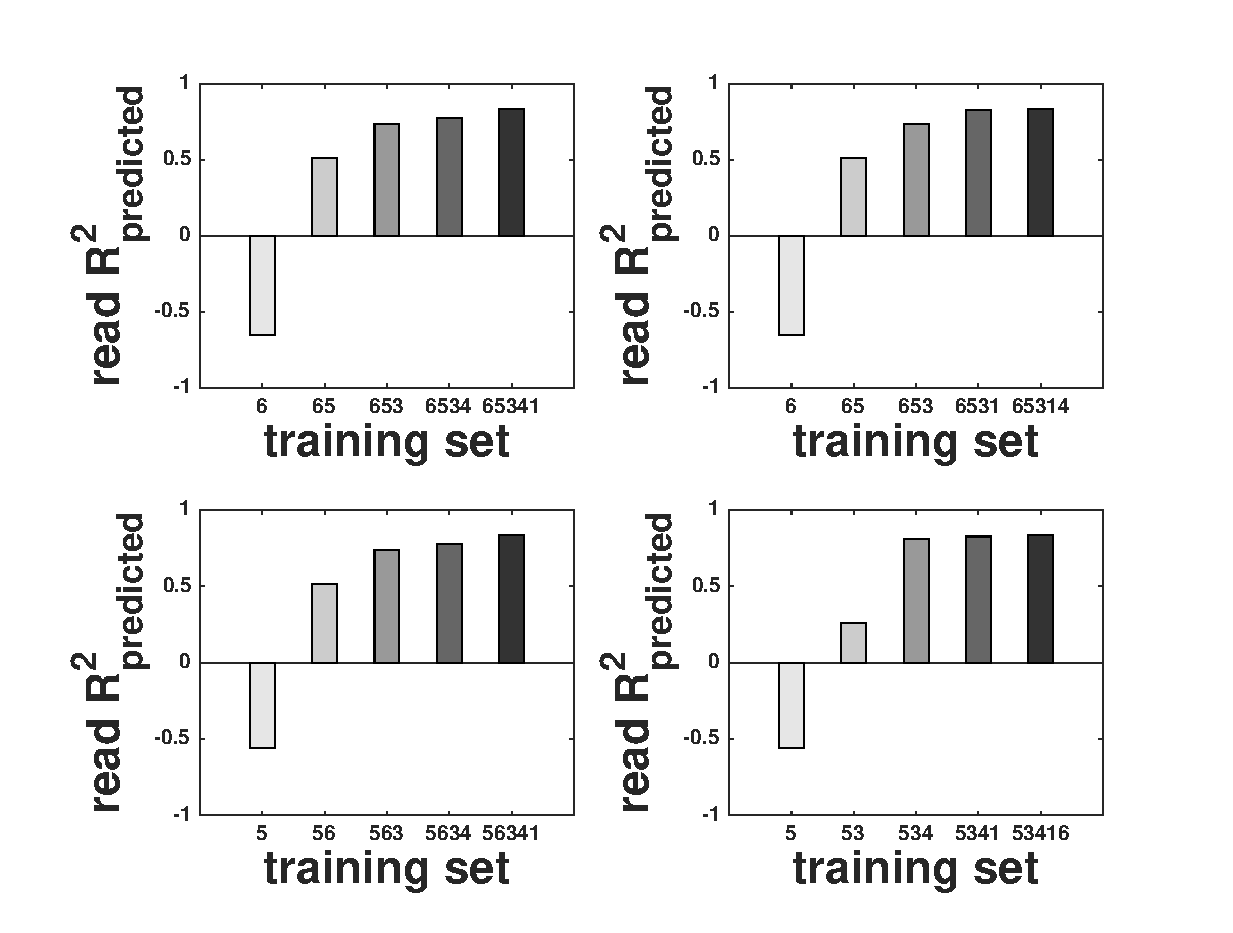
\includegraphics[scale = 0.5]{bar_read_avg_latency.eps}
    \caption{Redis read $R^2_{predicted}$ vs training set}
    \label{figure:redisbarread}
  \end{figure}

  \begin{figure}
    \centering
    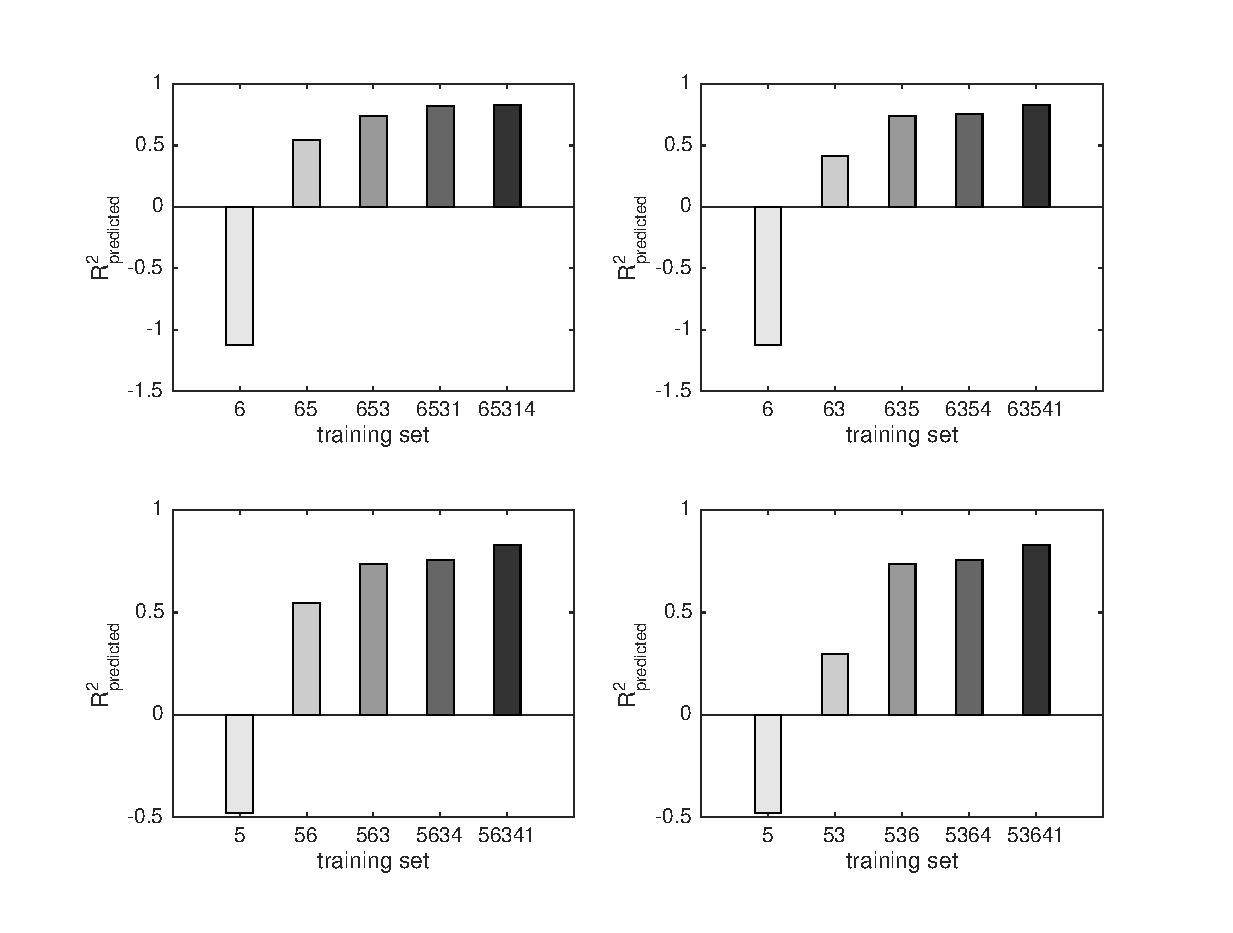
\includegraphics[scale = 0.5]{bar_write_avg_latency.eps}
    \caption{Redis write $R^2_{predicted}$ vs training set}
    \label{figure:redisbarwrite}
  \end{figure}

\begin{comment}

\begin{figure}[htbp]
\centering	
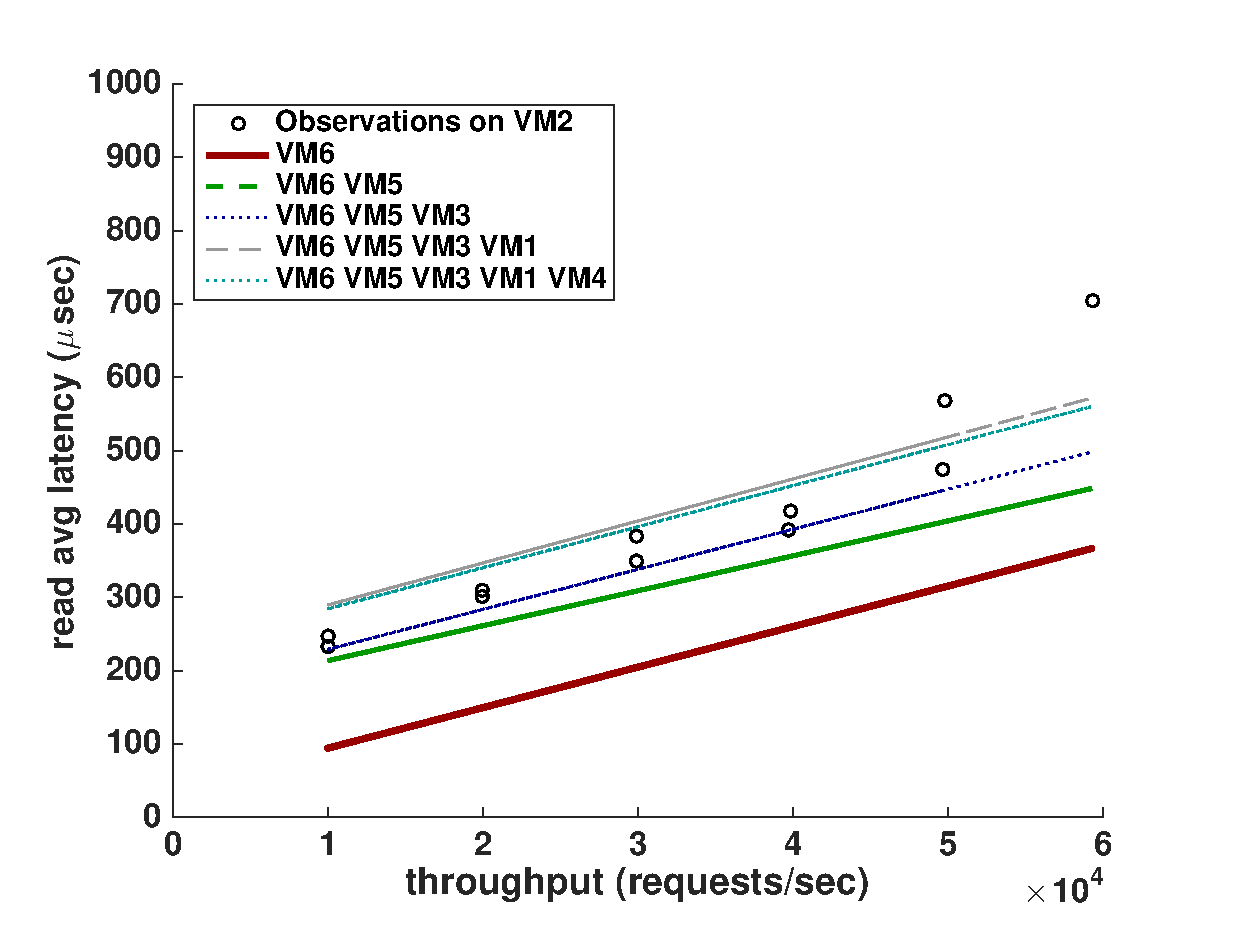
\includegraphics[width=0.45\textwidth]{fit_read_avg_latency_r3_2x_r3_x_m3_2x_m3__r3__m3_x.eps}
\caption{Redis average read latency vs throughput. ~\bu{TODO: cleanup plot formatting; make the numbers on the axes larger, label both the axes, use darker colors, move the box with names of providers to the top-left part of the graph.}}
\label{figure:redisbarread}
\end{figure}

\begin{figure}[htbp]
\centering	
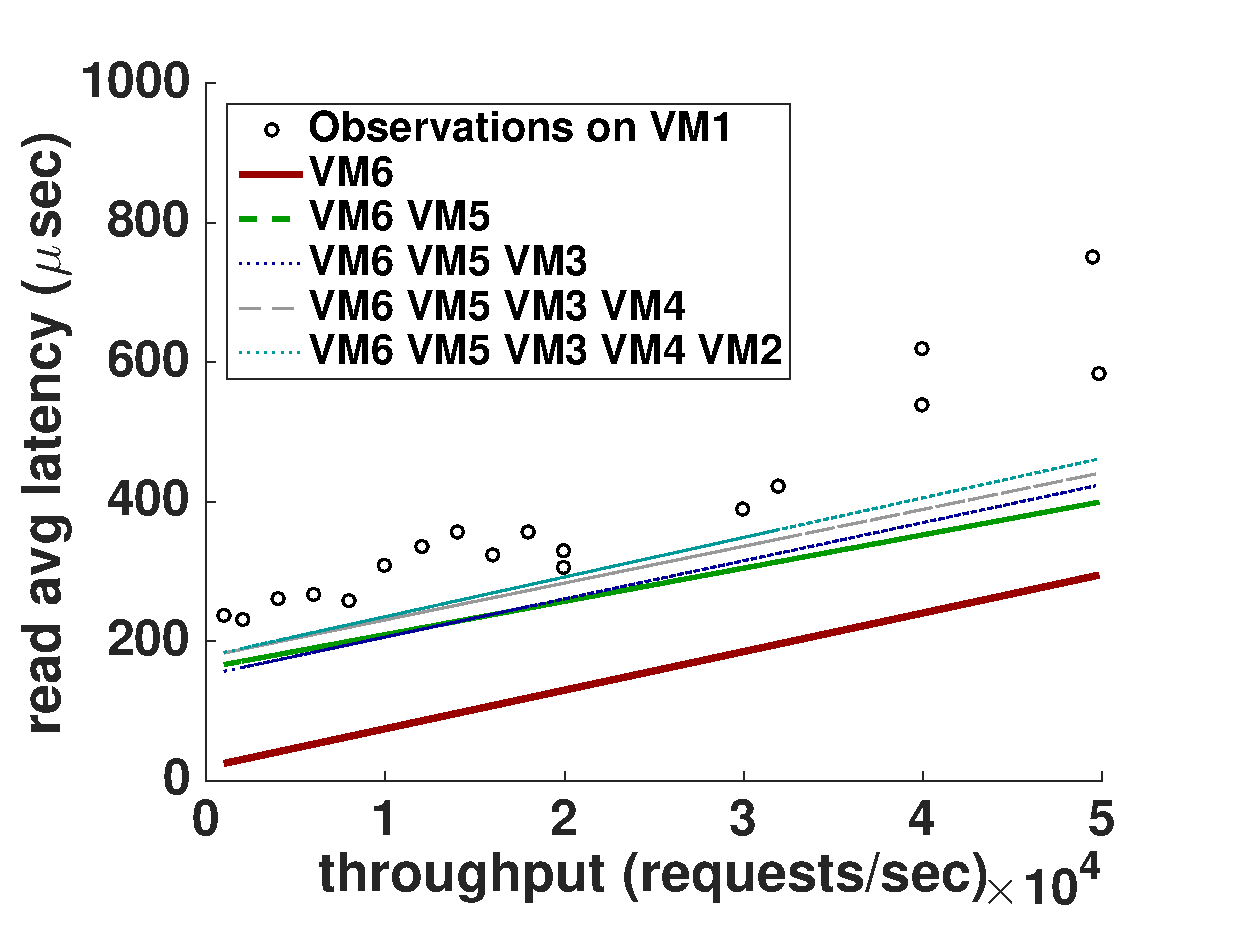
\includegraphics[width=0.45\textwidth]{fit_read_avg_latency_r3_2x_r3_x_m3_2x_r3__m3_x_m3_.eps}
\caption{Redis average read latency vs throughput. ~\bu{TODO: cleanup plot formatting; make the numbers on the axes larger, label both the axes, use darker colors, move the box with names of providers to the top-left part of the graph.}}
\label{figure:redisbarread}
\end{figure}

\begin{figure}[htbp]
\centering	
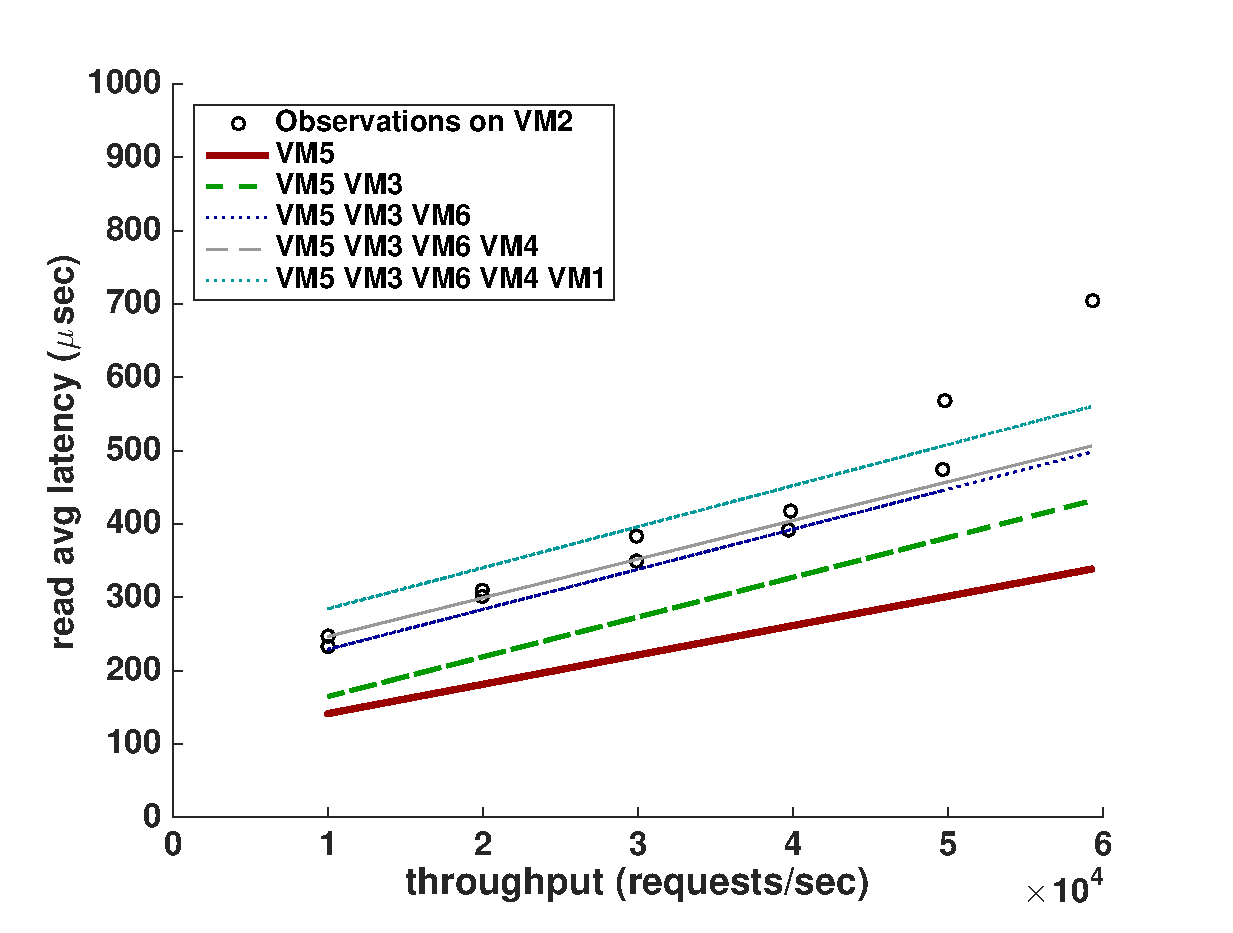
\includegraphics[width=0.45\textwidth]{fit_read_avg_latency_r3_x_m3_2x_r3_2x_r3__m3__m3_x.eps}
\caption{Redis average read latency vs throughput. ~\bu{TODO: cleanup plot formatting; make the numbers on the axes larger, label both the axes, use darker colors, move the box with names of providers to the top-left part of the graph.}}
\label{figure:redisbarread}
\end{figure}

\begin{figure}[htbp]
\centering	
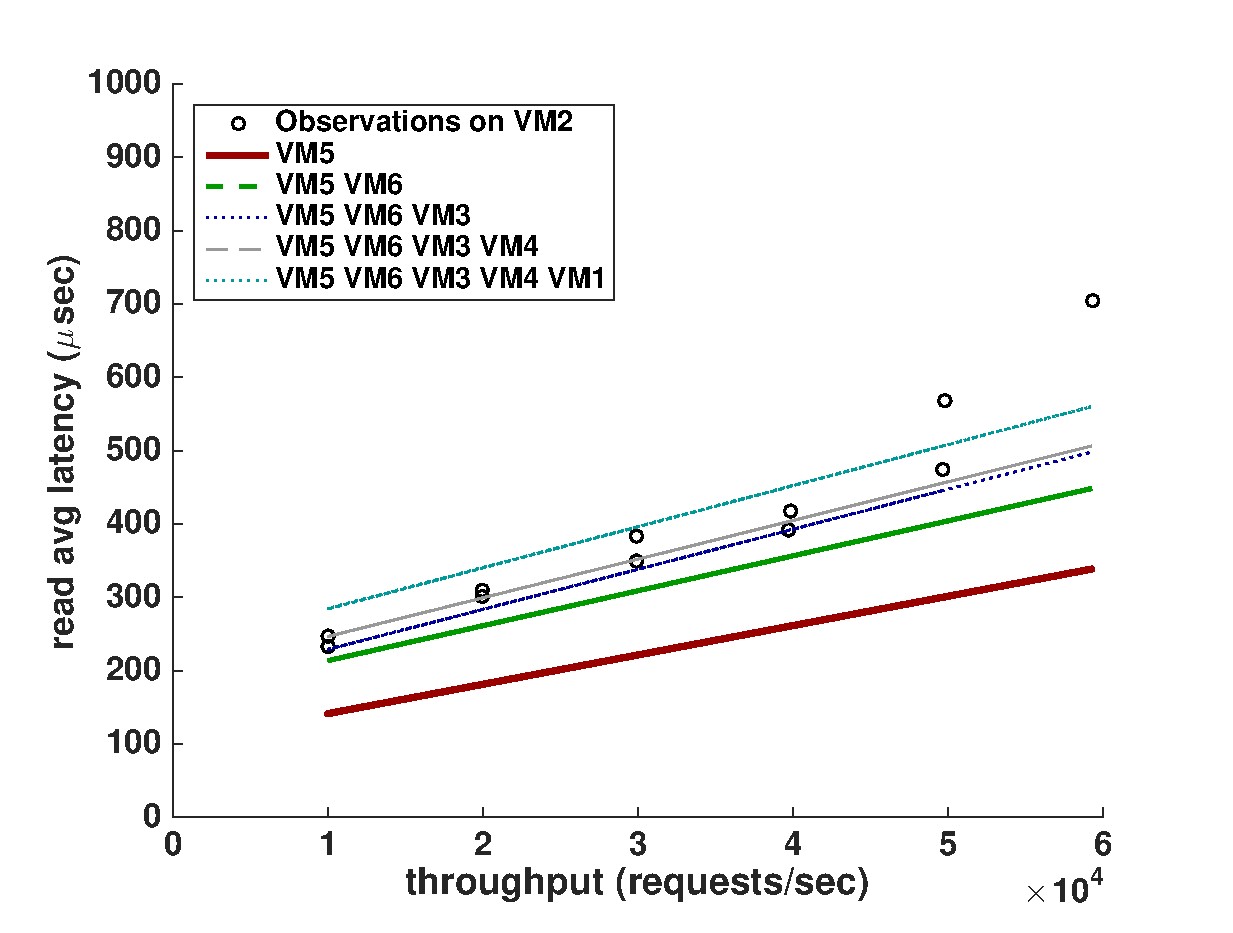
\includegraphics[width=0.45\textwidth]{fit_read_avg_latency_r3_x_r3_2x_m3_2x_r3__m3__m3_x.eps}
\caption{Redis average read latency vs throughput. ~\bu{TODO: cleanup plot formatting; make the numbers on the axes larger, label both the axes, use darker colors, move the box with names of providers to the top-left part of the graph.}}
\label{figure:redisbarread}
\end{figure}

%\begin{figure}[t]
%\twobytwofig{fit_read_avg_latency_r3_2x_r3_x_m3_2x_m3__r3__m3_x.eps}{}
%{fit_read_avg_latency_r3_2x_r3_x_m3_2x_r3__m3_x_m3_.eps}{}
%{fit_read_avg_latency_r3_x_m3_2x_r3_2x_r3__m3__m3_x.eps}{}
%{fit_read_avg_latency_r3_x_r3_2x_m3_2x_r3__m3__m3_x.eps}{}
%\caption{Profiles of Various Server Applications}
%\label{fig:redisread}
%\end{figure}

\end{comment}

\begin{figure*}[t]
\subfloat[fig 1]{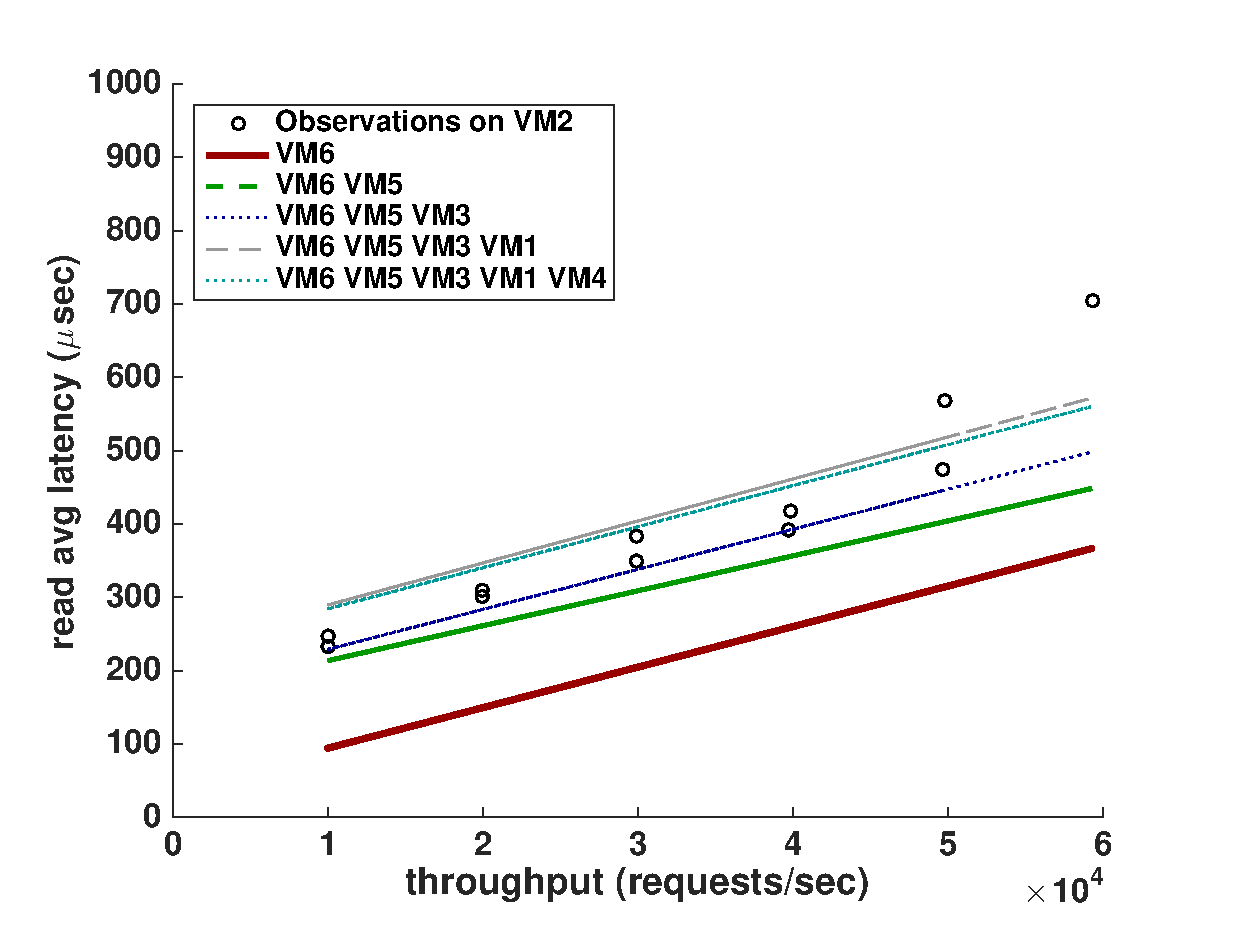
\includegraphics[width=0.5\textwidth]{fit_read_avg_latency_r3_2x_r3_x_m3_2x_m3__r3__m3_x}} 
\subfloat[fig 2]{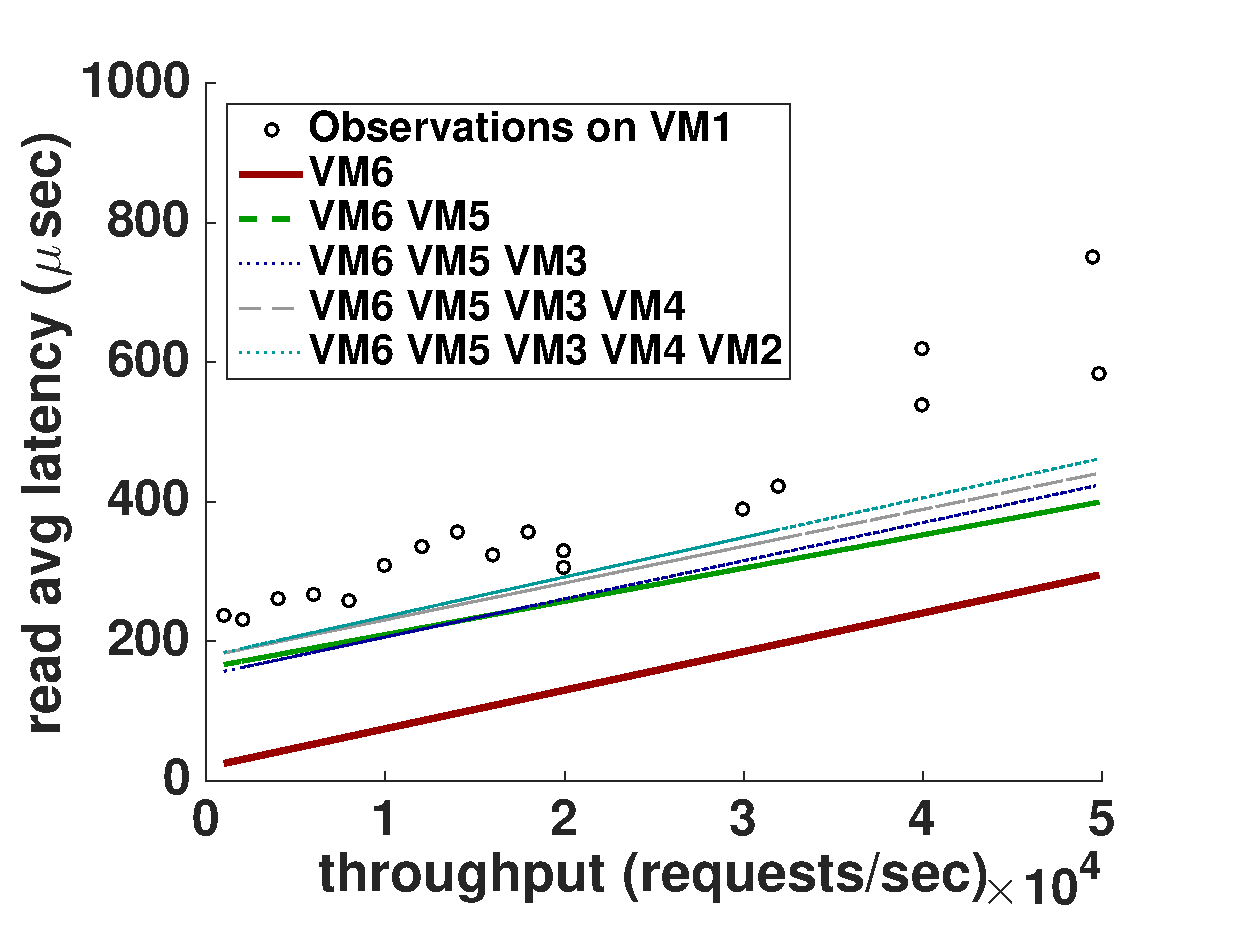
\includegraphics[width=0.5\textwidth]{fit_read_avg_latency_r3_2x_r3_x_m3_2x_r3__m3_x_m3_}}\\
\subfloat[fig 3]{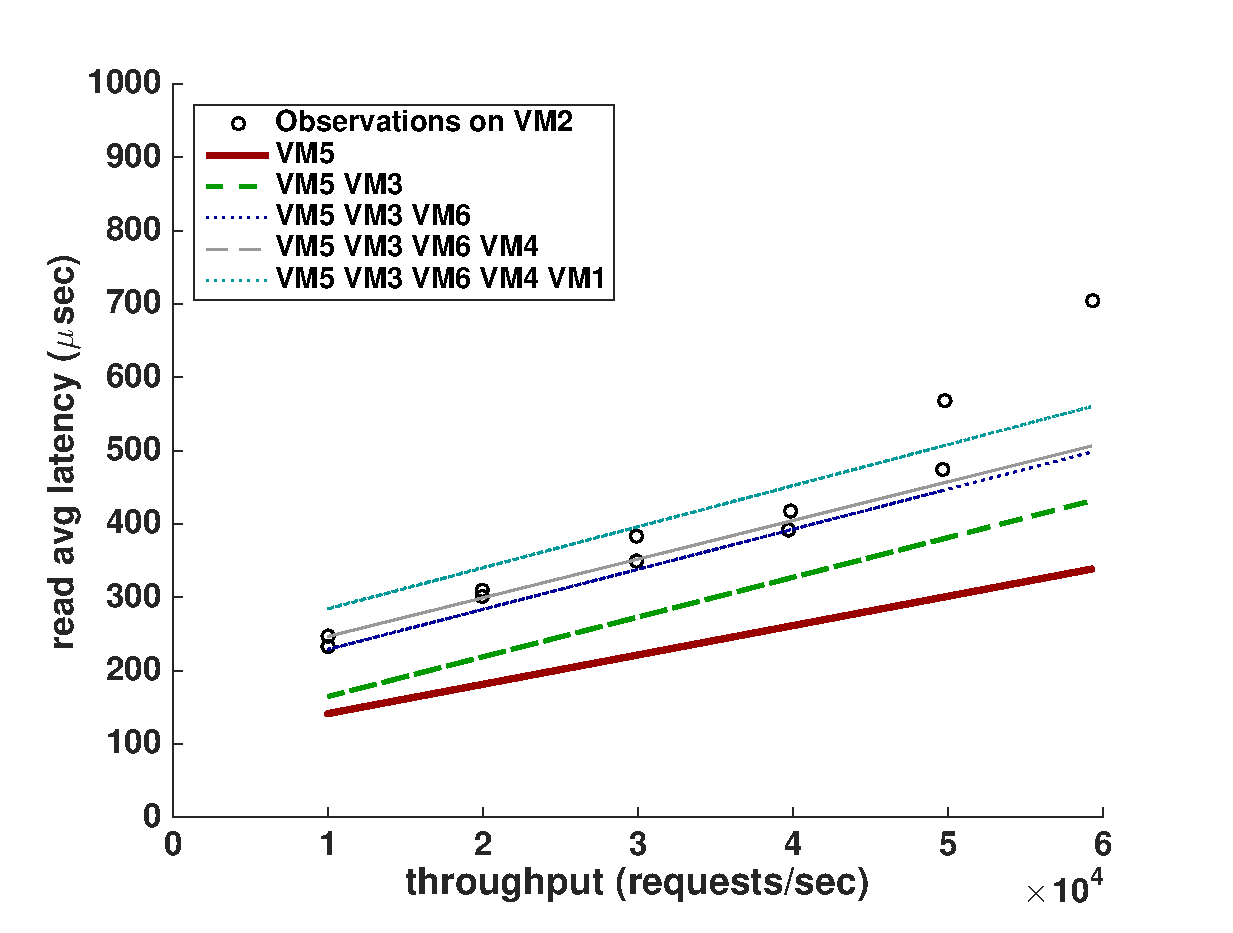
\includegraphics[width=0.5\textwidth]{fit_read_avg_latency_r3_x_m3_2x_r3_2x_r3__m3__m3_x.eps}}
\subfloat[fig 4]{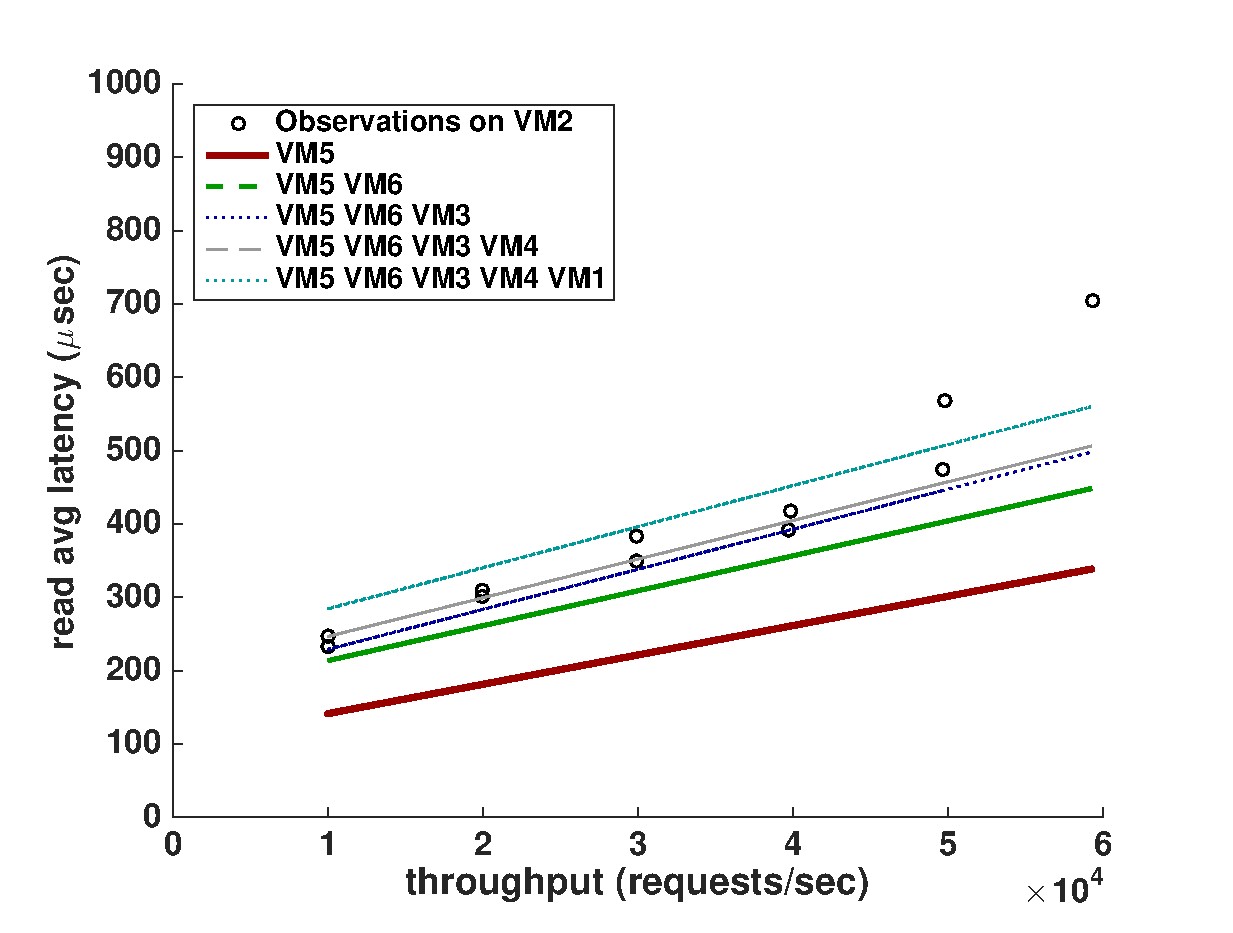
\includegraphics[width=0.5\textwidth]{fit_read_avg_latency_r3_x_r3_2x_m3_2x_r3__m3__m3_x.eps}} 
\caption{Incremental fit for Redis Average Read Latency }
\label{figure:redisfitread}
\end{figure*}

%%%%%%%%%%%%

\begin{comment}

\begin{figure}[htbp]
\centering	
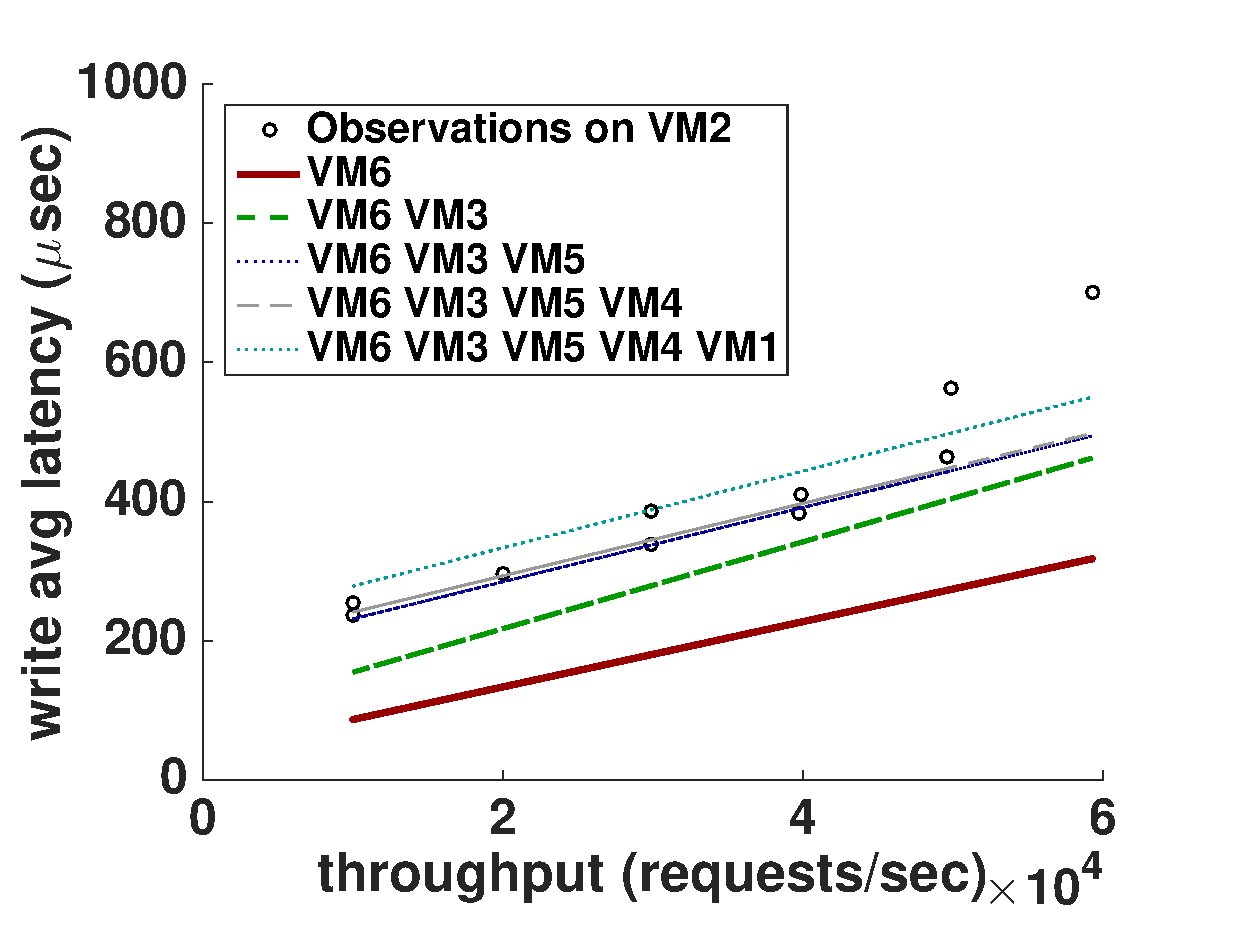
\includegraphics[width=0.45\textwidth]{fit_write_avg_latency_r3_2x_m3_2x_r3_x_r3__m3__m3_x.eps}
\caption{Redis average write latency vs throughput. ~\bu{TODO: cleanup plot formatting; make the numbers on the axes larger, label both the axes, use darker colors, move the box with names of providers to the top-left part of the graph.}}
\label{figure:redisbarread}
\end{figure}

\begin{figure}[htbp]
\centering	
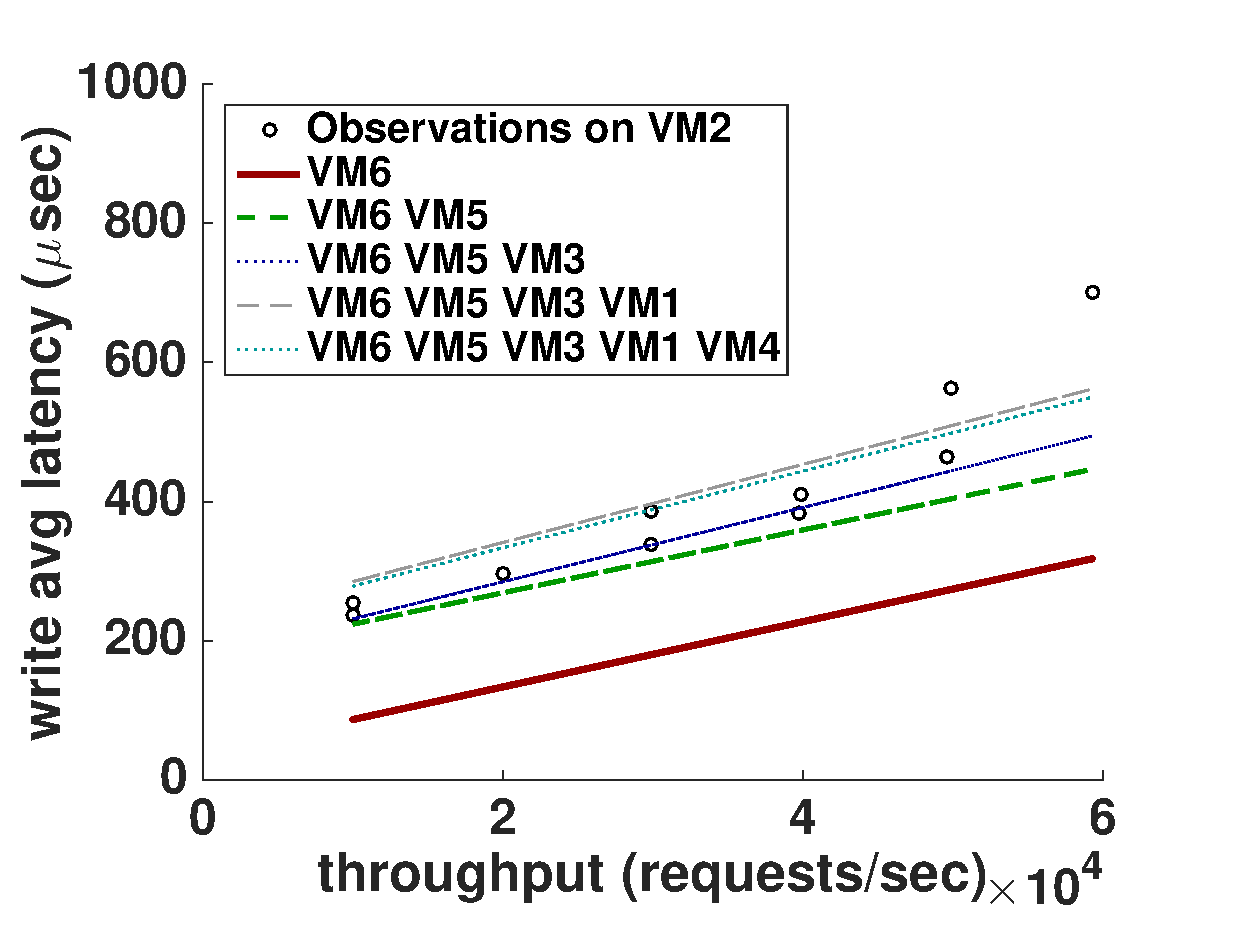
\includegraphics[width=0.45\textwidth]{fit_write_avg_latency_r3_2x_r3_x_m3_2x_m3__r3__m3_x.eps}
\caption{Redis average write latency vs throughput. ~\bu{TODO: cleanup plot formatting; make the numbers on the axes larger, label both the axes, use darker colors, move the box with names of providers to the top-left part of the graph.}}
\label{figure:redisbarread}
\end{figure}

\begin{figure}[htbp]
\centering	
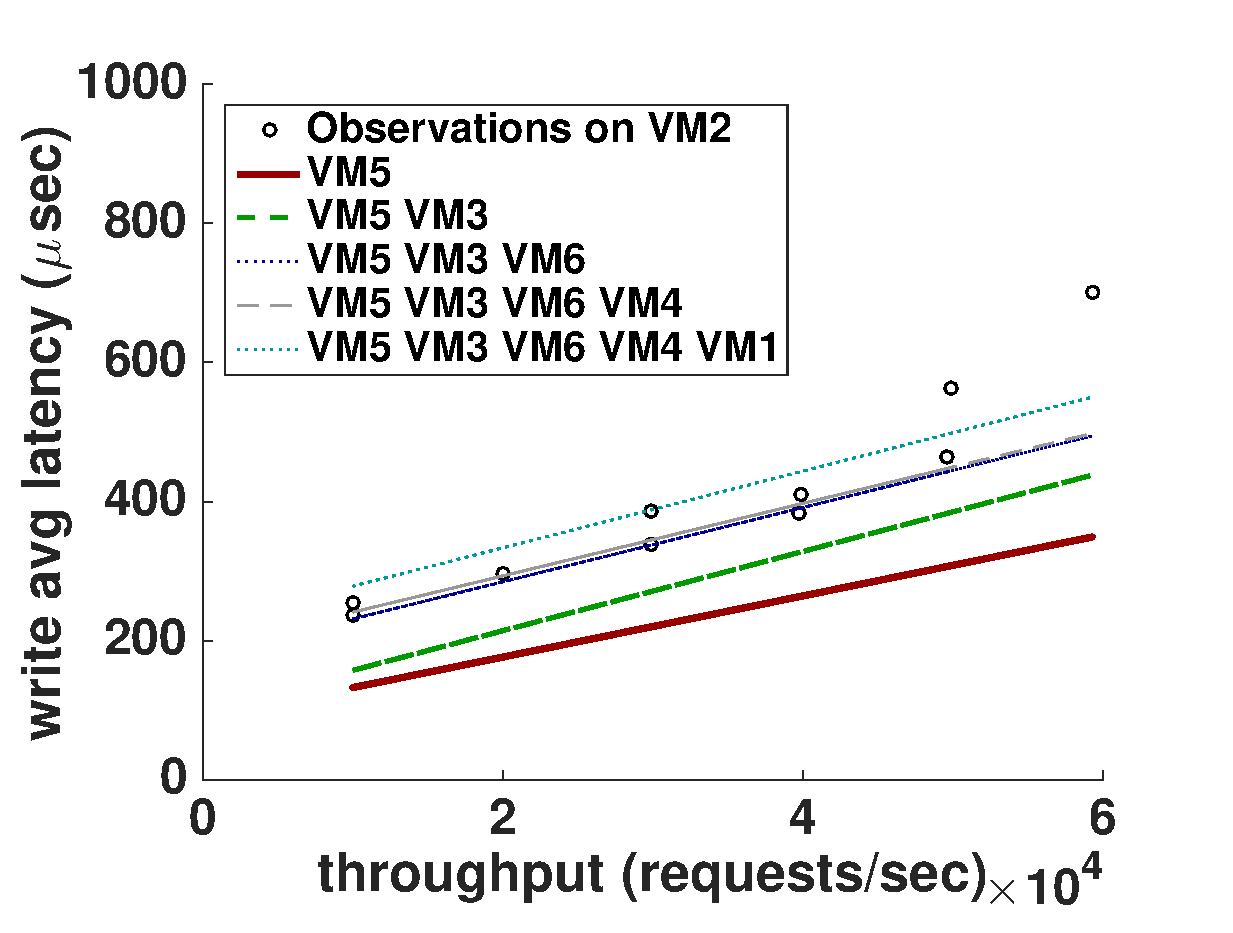
\includegraphics[width=0.45\textwidth]{fit_write_avg_latency_r3_x_m3_2x_r3_2x_r3__m3__m3_x.eps}
\caption{Redis average write latency vs throughput. ~\bu{TODO: cleanup plot formatting; make the numbers on the axes larger, label both the axes, use darker colors, move the box with names of providers to the top-left part of the graph.}}
\label{figure:redisbarread}
\end{figure}

\begin{figure}[htbp]
\centering	
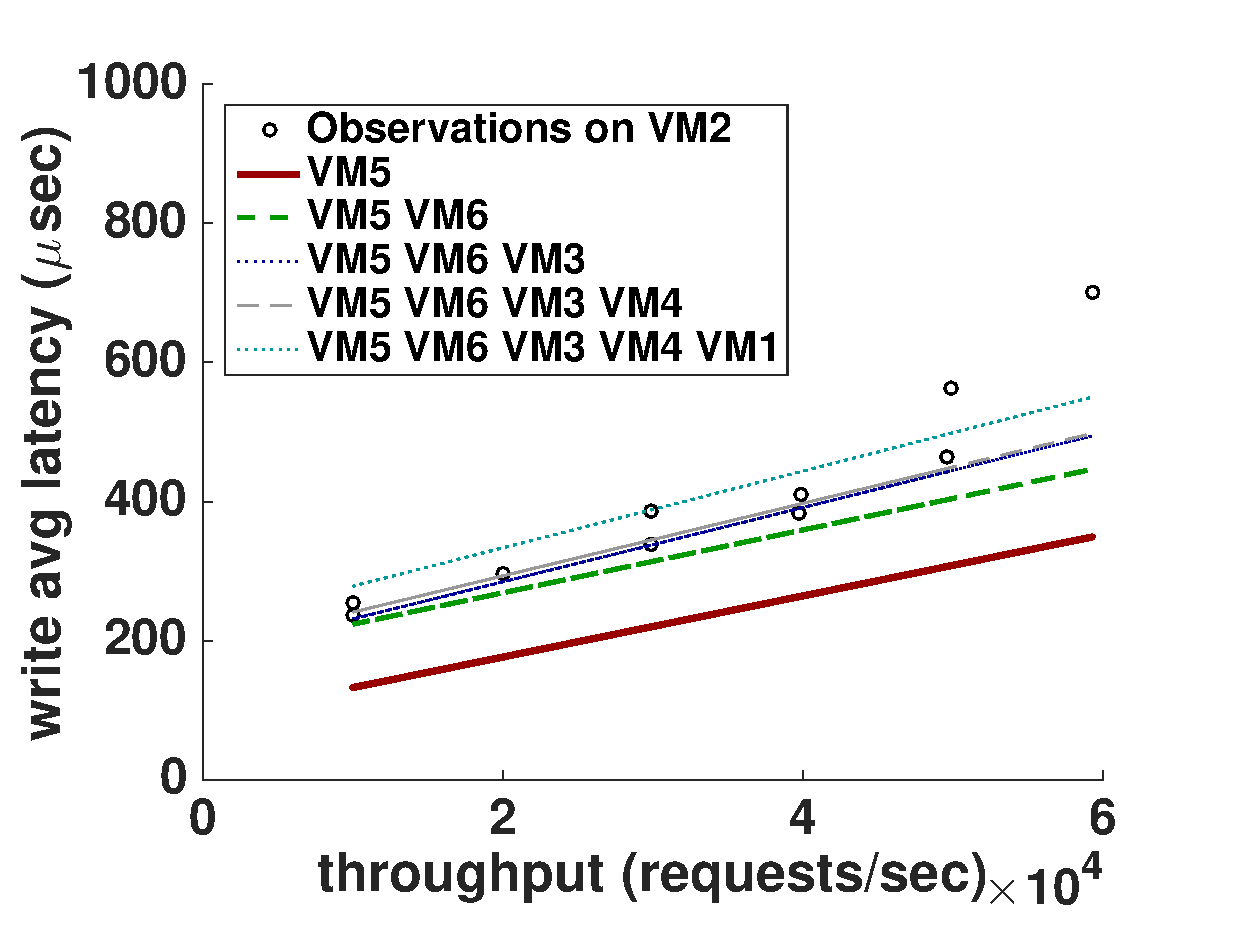
\includegraphics[width=0.45\textwidth]{fit_write_avg_latency_r3_x_r3_2x_m3_2x_r3__m3__m3_x.eps}
\caption{Redis average write latency vs throughput. ~\bu{TODO: cleanup plot formatting; make the numbers on the axes larger, label both the axes, use darker colors, move the box with names of providers to the top-left part of the graph.}}
\label{figure:redisbarread}
\end{figure}
\end{comment}

\begin{figure*}[t]
\subfloat[fig 1]{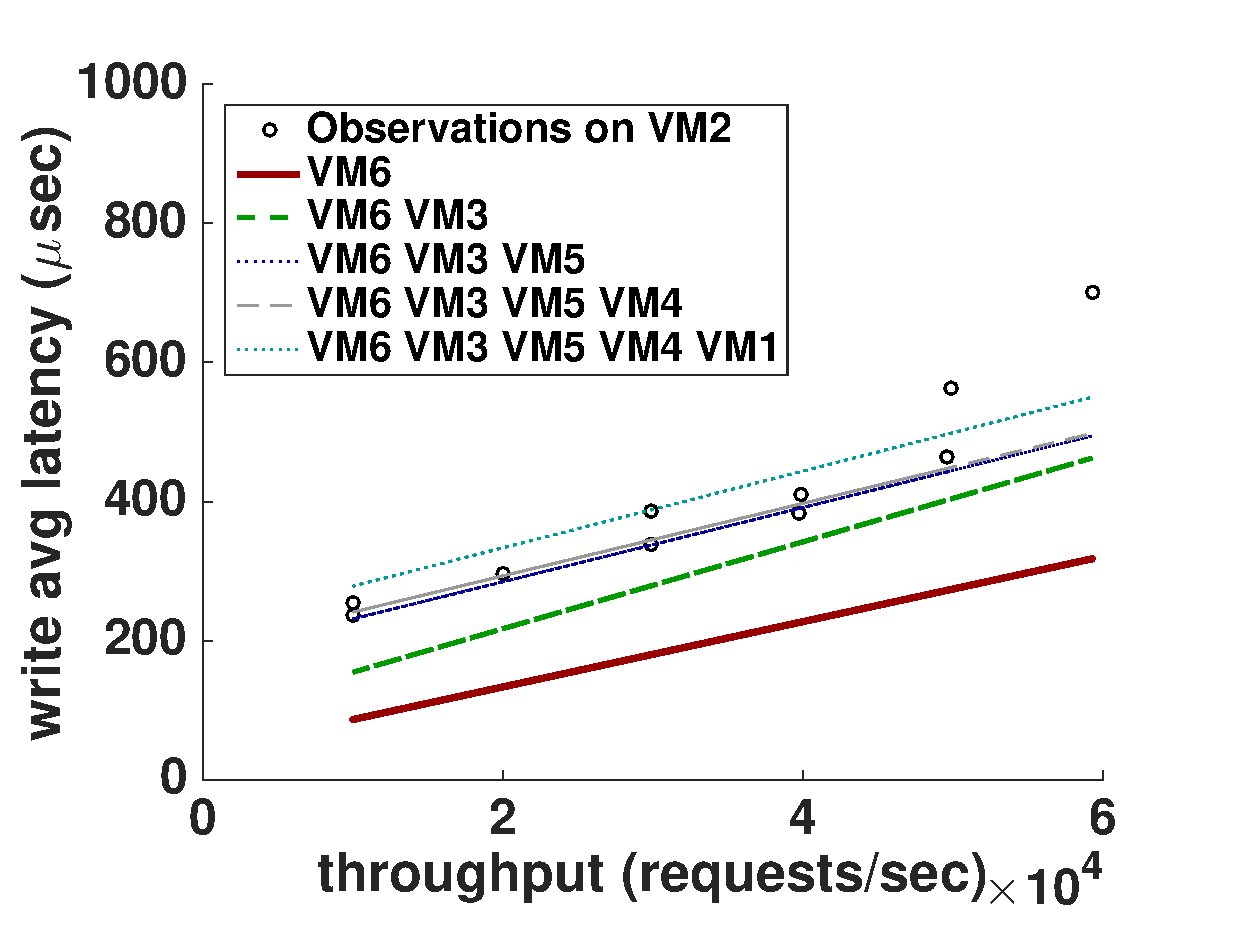
\includegraphics[width=0.5\textwidth]{fit_write_avg_latency_r3_2x_m3_2x_r3_x_r3__m3__m3_x.eps}} 
\subfloat[fig 2]{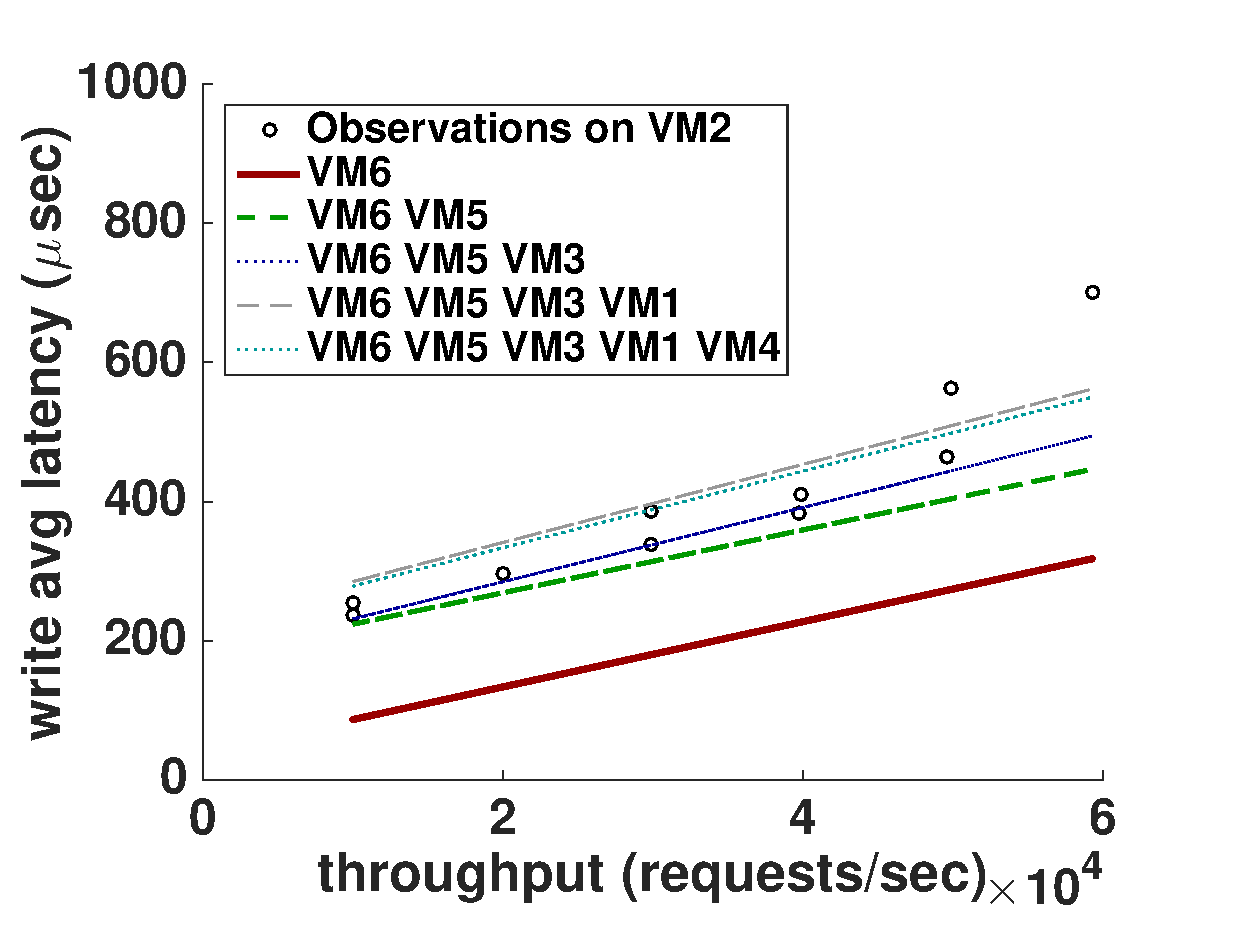
\includegraphics[width=0.5\textwidth]{fit_write_avg_latency_r3_2x_r3_x_m3_2x_m3__r3__m3_x.eps}}\\
\subfloat[fig 3]{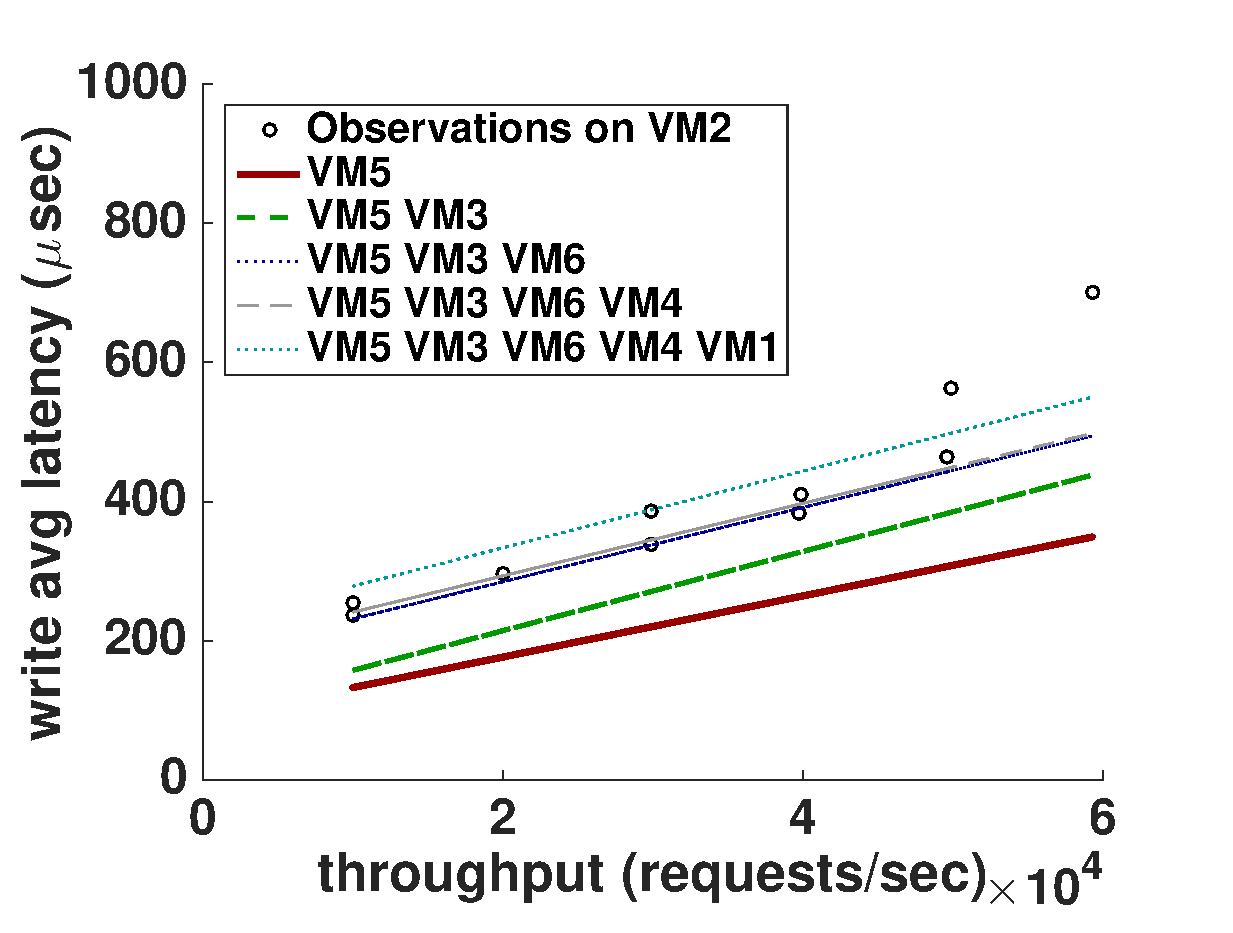
\includegraphics[width=0.5\textwidth]{fit_write_avg_latency_r3_x_m3_2x_r3_2x_r3__m3__m3_x.eps}}
\subfloat[fig 4]{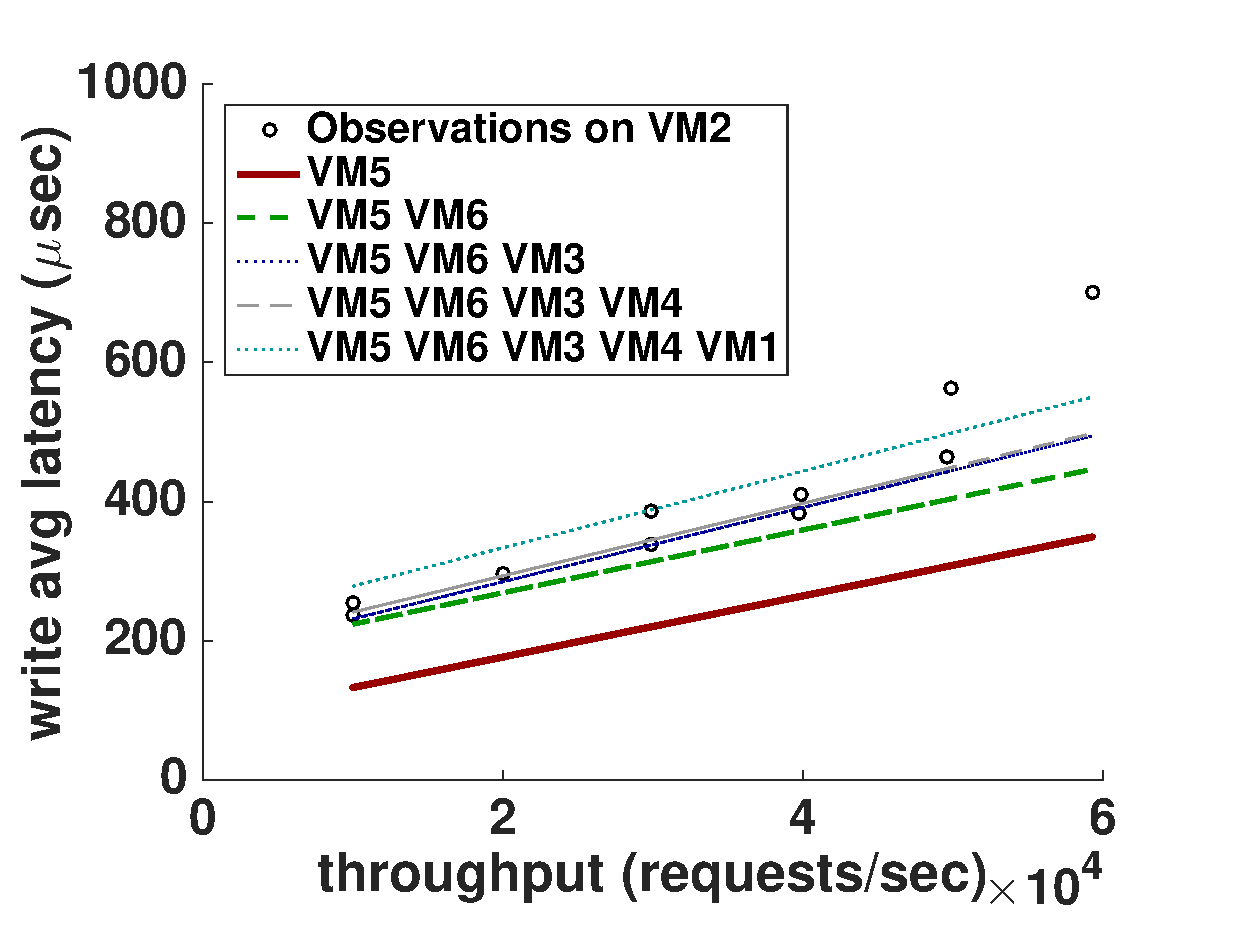
\includegraphics[width=0.5\textwidth]{fit_write_avg_latency_r3_x_r3_2x_m3_2x_r3__m3__m3_x.eps}} 
\caption{Incremental fit for Redis Average Write Latency }
\label{figure:redisfitwrite}
\end{figure*}

\subsection{Case Study 2: Apache Cassandra}
\vspace{10pt}

\mm{
Apache Cassandra is a Table/Key-Value hybrid NoSQL database.  It is suitable for applications that require high availability provided by replication.  In terms of the CAP theorem, Cassandra prioritizes availability and performance over consistency, making it highly performant and scalable, though consistency is eventual rather than strong, for typical Cassandra applications.
 
Apache Cassandra was installed on Amazon EC2 instances of various VM instance types.  Our testing was done on Cassandra clusters with 5 nodes.  We ran our testing with a replication factor of three, so every database record was stored on three of the five nodes.  We tested using weak (or eventual) consistency, using a consistency level of "ONE".

We ran the YCSB client on a m4.2xlarge EC2 instance running Ubuntu Linux 14.04. We monitored the system load average on the client machine to verify that the client was not the bottleneck during the tests.
}

\begin{comment}
  \begin{figure}
  \centering
    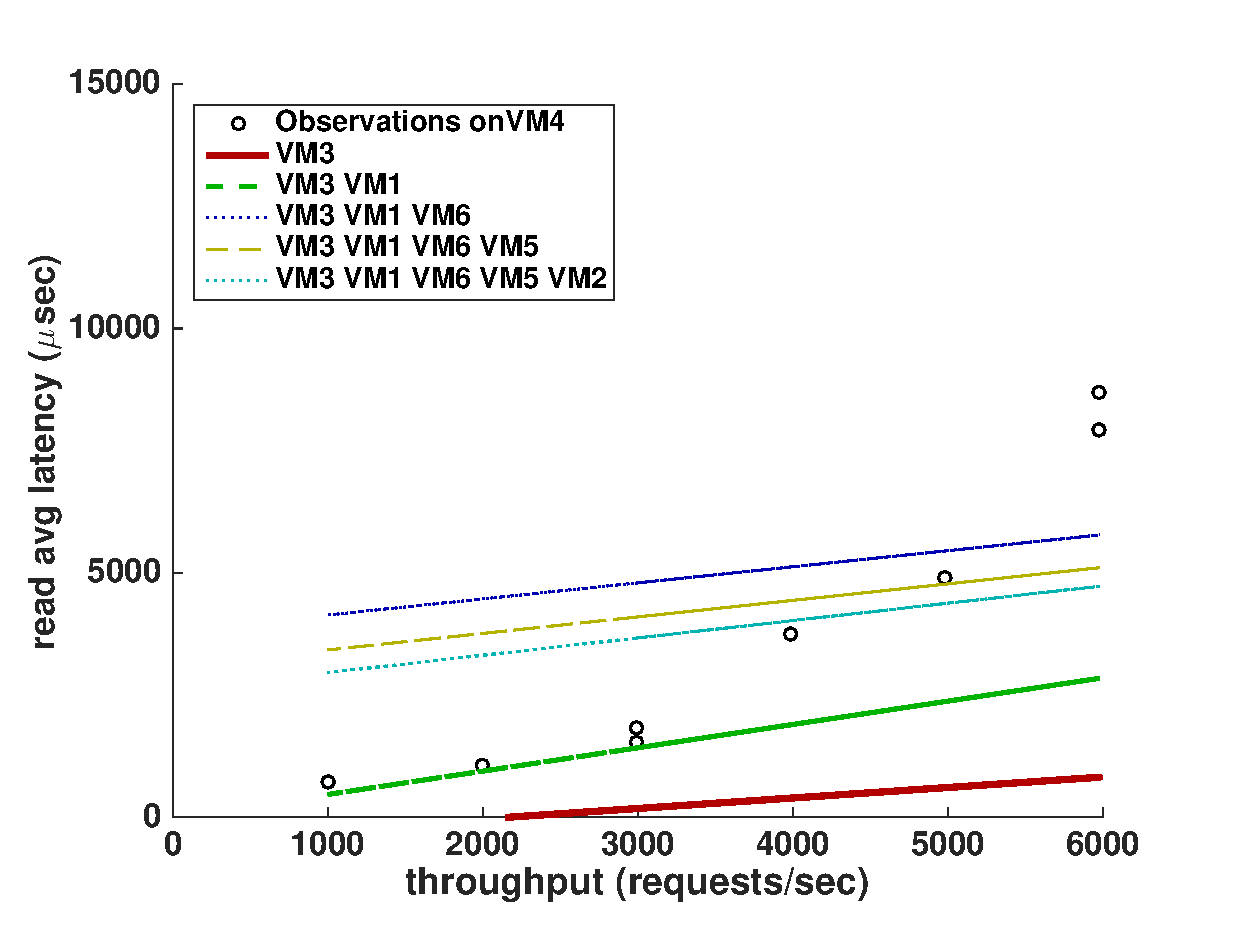
\includegraphics[scale = 0.25]{cassandra_fit_read_avg_latency_m3_2x_m3__r3_2x_r3_x_m3_x_r3_.eps}
    \caption{Cassandra average read latency vs throughput}
    \label{figure:redisbarread}
  \end{figure}

  \begin{figure}
  \centering
    \includegraphics[scale = 0.25]{cassandra_fit_read_avg_latency_r3_2x_r3_x_m3_x_m3__m3_2x_r3_.eps}
    \caption{Cassandra average read latency vs throughput}
    \label{figure:redisbarread}
  \end{figure}

  \begin{figure}
  \centering
    \includegraphics[scale = 0.25]{cassandra_fit_read_avg_latency_r3__m3_x_r3_2x_m3_2x_r3_x_m3_.eps}
    \caption{Cassandra average read latency vs throughput}
    \label{figure:redisbarread}
  \end{figure}

  \begin{figure}
  \centering
    \includegraphics[scale = 0.25]{cassandra_fit_read_avg_latency_r3_x_m3__r3_2x_m3_x_m3_2x_r3_.eps}
    \caption{Cassandra average read latency vs throughput}
    \label{figure:redisbarread}
  \end{figure}
\end{comment}

\begin{figure*}[t]
\subfloat[fig 1]{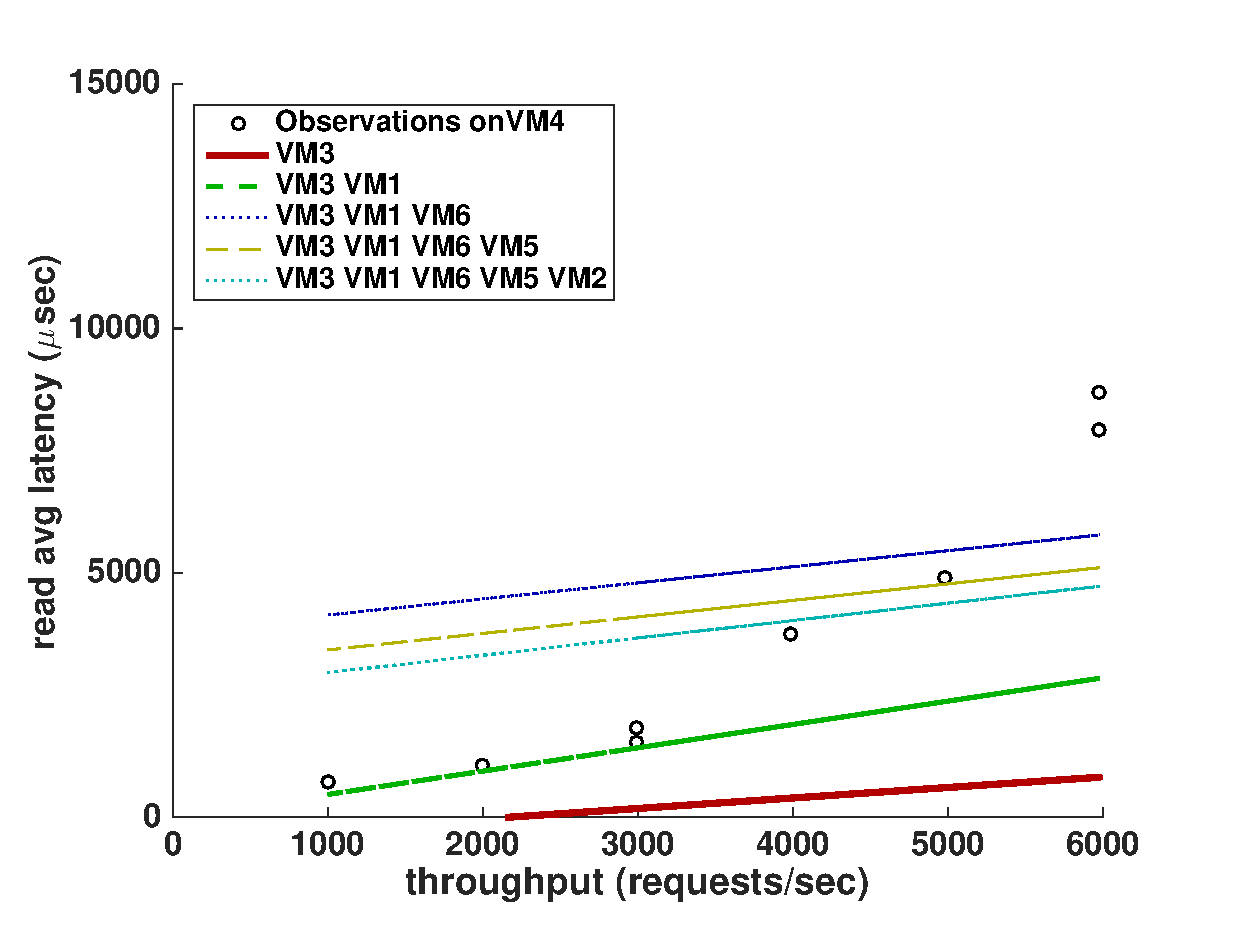
\includegraphics[width=0.5\textwidth]{cassandra_fit_read_avg_latency_m3_2x_m3__r3_2x_r3_x_m3_x_r3_.eps}} 
\subfloat[fig 2]{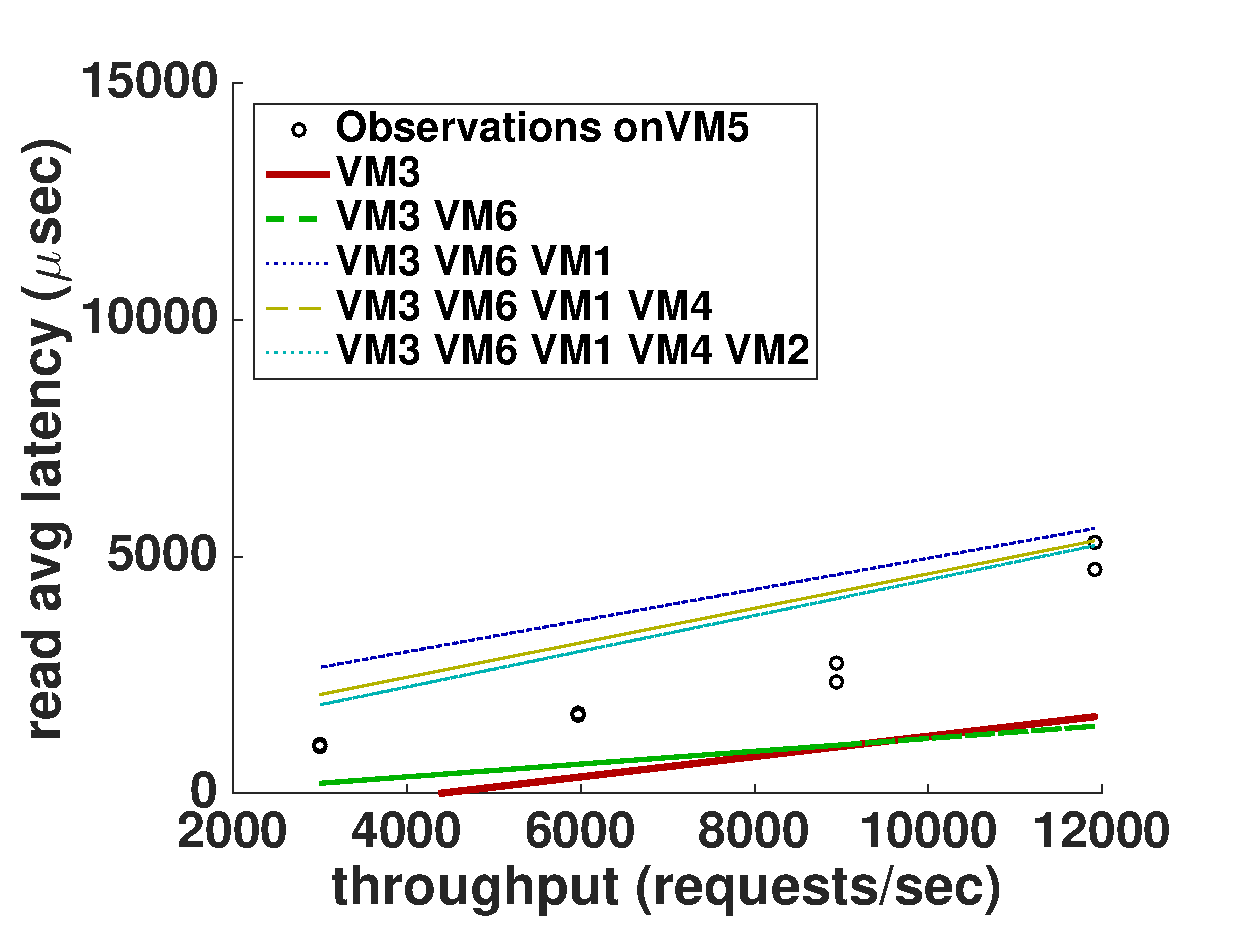
\includegraphics[width=0.5\textwidth]{cassandra_fit_read_avg_latency_m3_2x_r3_2x_m3__r3__m3_x_r3_x.eps}}\\
\subfloat[fig 3]{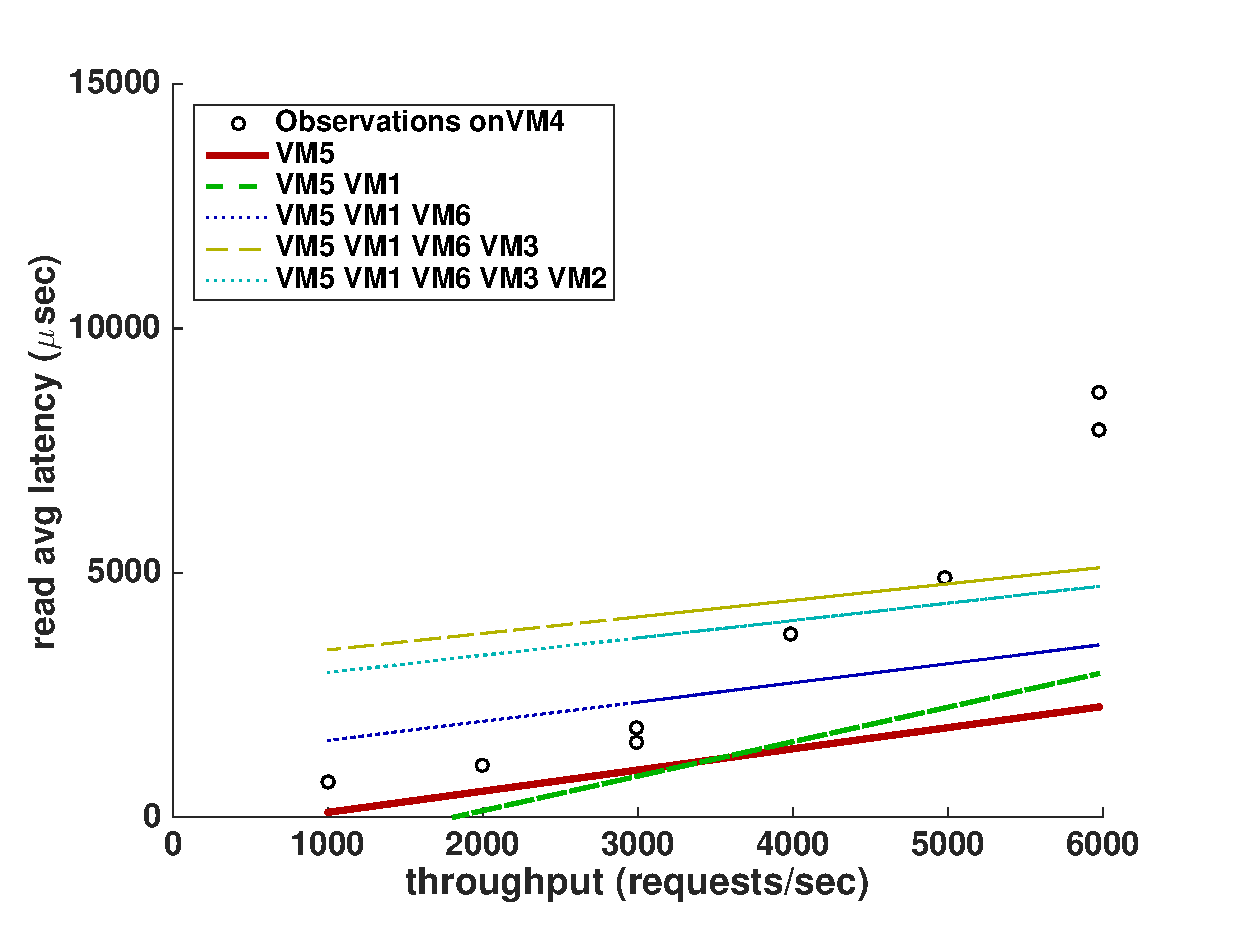
\includegraphics[width=0.5\textwidth]{cassandra_fit_read_avg_latency_r3_x_m3__r3_2x_m3_2x_m3_x_r3_.eps}}
\subfloat[fig 4]{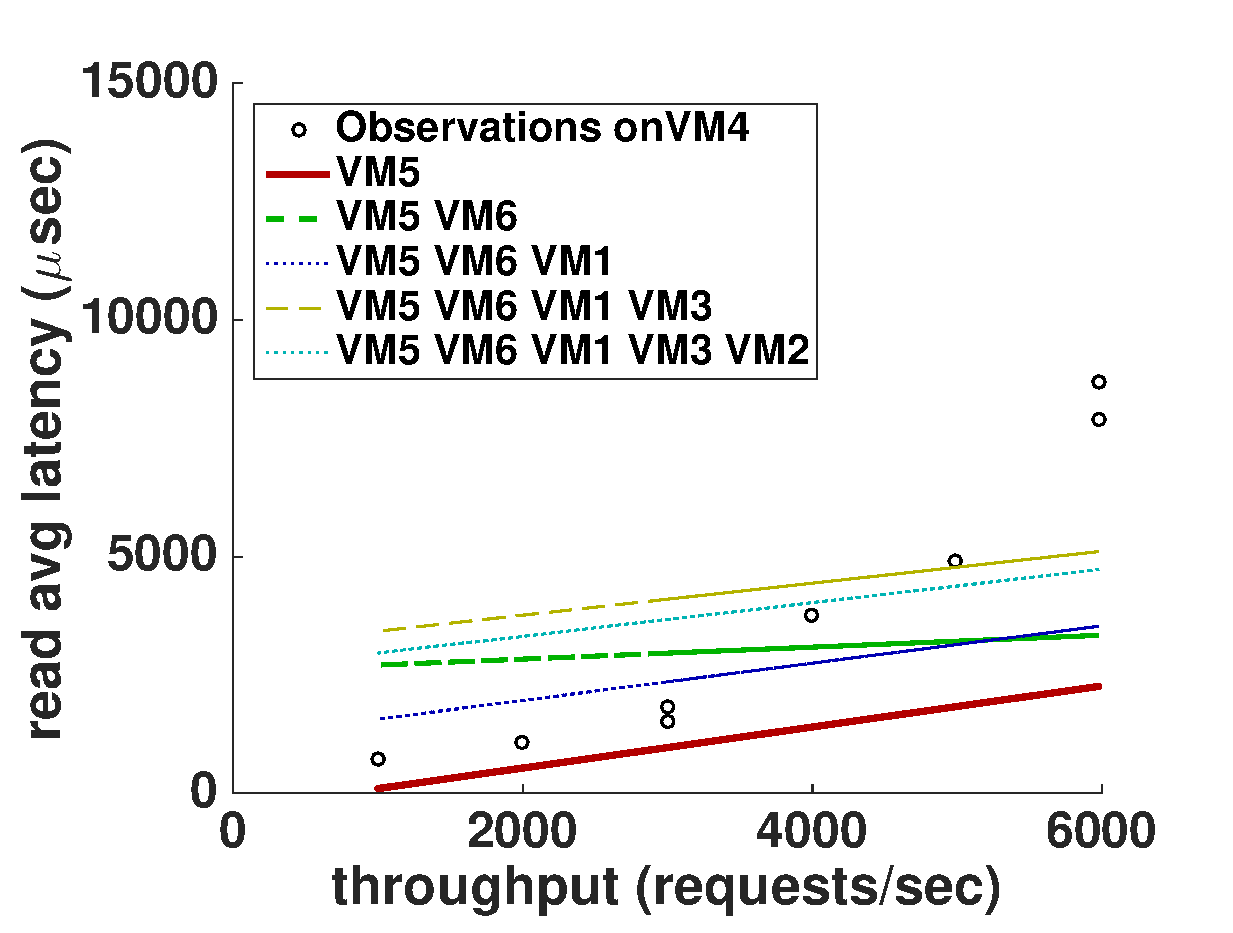
\includegraphics[width=0.5\textwidth]{cassandra_fit_read_avg_latency_r3_x_r3_2x_m3__m3_2x_m3_x_r3_.eps}}
\caption{Incremental fit for Cassandra Average Read Latency }
\label{some example}
\end{figure*}

\begin{comment}
  \begin{figure}
  \centering
    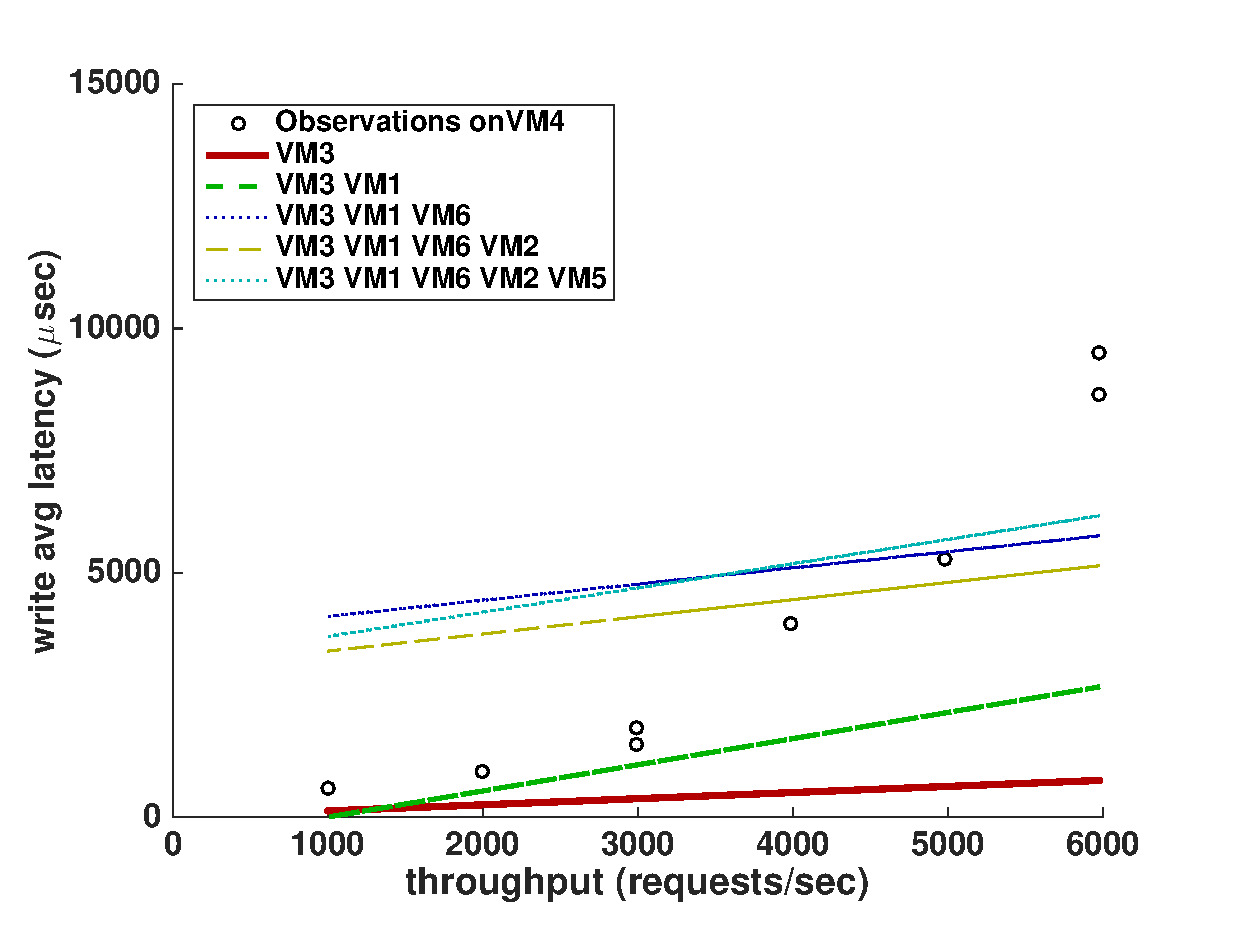
\includegraphics[scale = 0.25]{cassandra_fit_write_avg_latency_m3_2x_m3__r3_2x_m3_x_r3_x_r3_.eps}
    \caption{Cassandra average read latency vs throughput}
    \label{figure:redisbarread}
  \end{figure}

  \begin{figure}
  \centering
    \includegraphics[scale = 0.25]{cassandra_fit_write_avg_latency_m3_2x_m3_x_r3__r3_2x_r3_x_m3_.eps}
    \caption{Cassandra average read latency vs throughput}
    \label{figure:redisbarread}
  \end{figure}

  \begin{figure}
  \centering
    \includegraphics[scale = 0.25]{cassandra_fit_write_avg_latency_m3_2x_r3_x_r3_2x_m3_x_r3__m3_.eps}
    \caption{Cassandra average write latency vs throughput}
    \label{figure:redisbarread}
  \end{figure}

  \begin{figure}
  \centering
    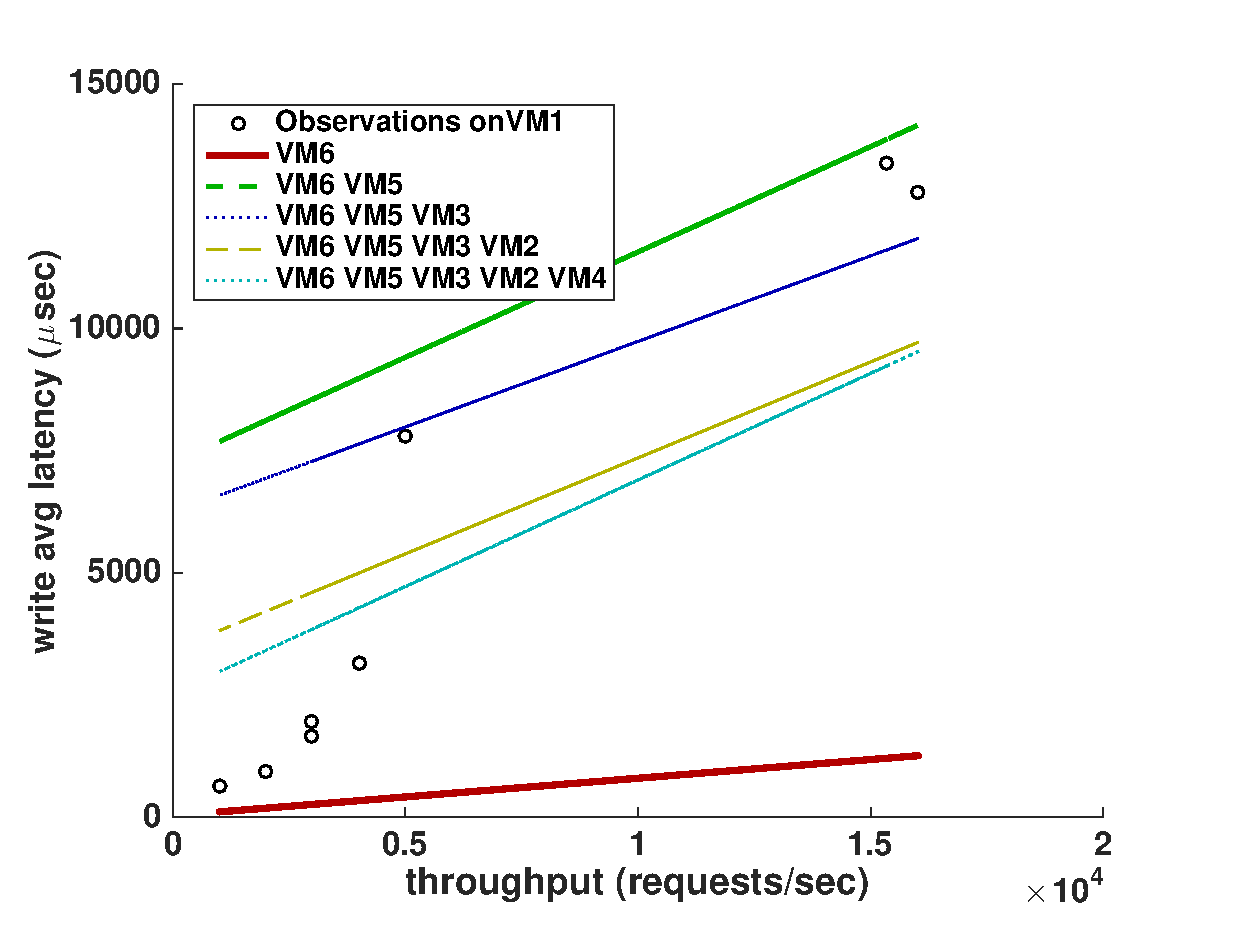
\includegraphics[scale = 0.25]{cassandra_fit_write_avg_latency_r3_2x_r3_x_m3_2x_m3_x_r3__m3_.eps}
    \caption{Cassandra average write latency vs throughput}
    \label{figure:redisbarread}
  \end{figure}
\end{comment}

\begin{figure*}[t]
\subfloat[fig 1]{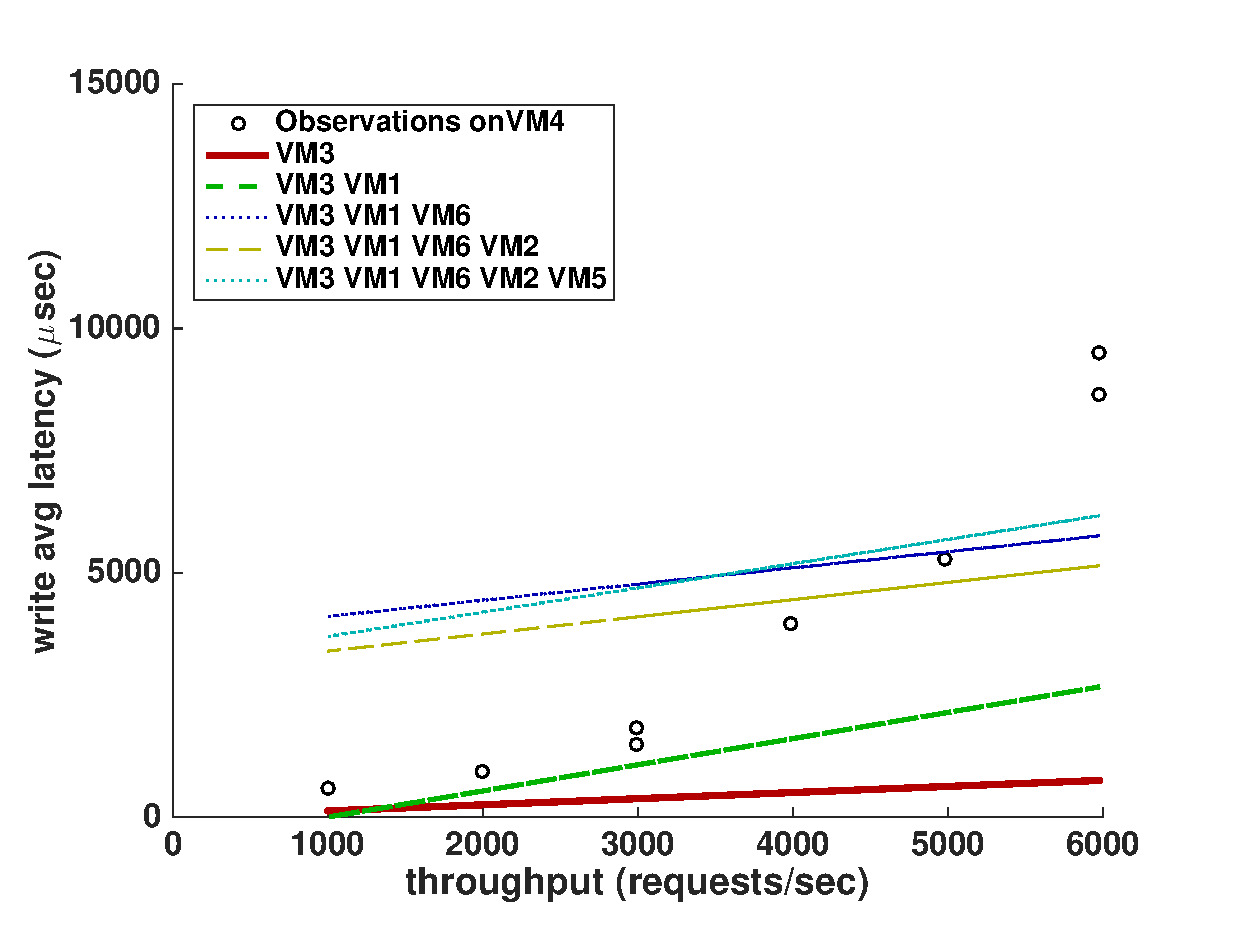
\includegraphics[width=0.5\textwidth]{cassandra_fit_write_avg_latency_m3_2x_m3__r3_2x_m3_x_r3_x_r3_.eps}} 
\subfloat[fig 2]{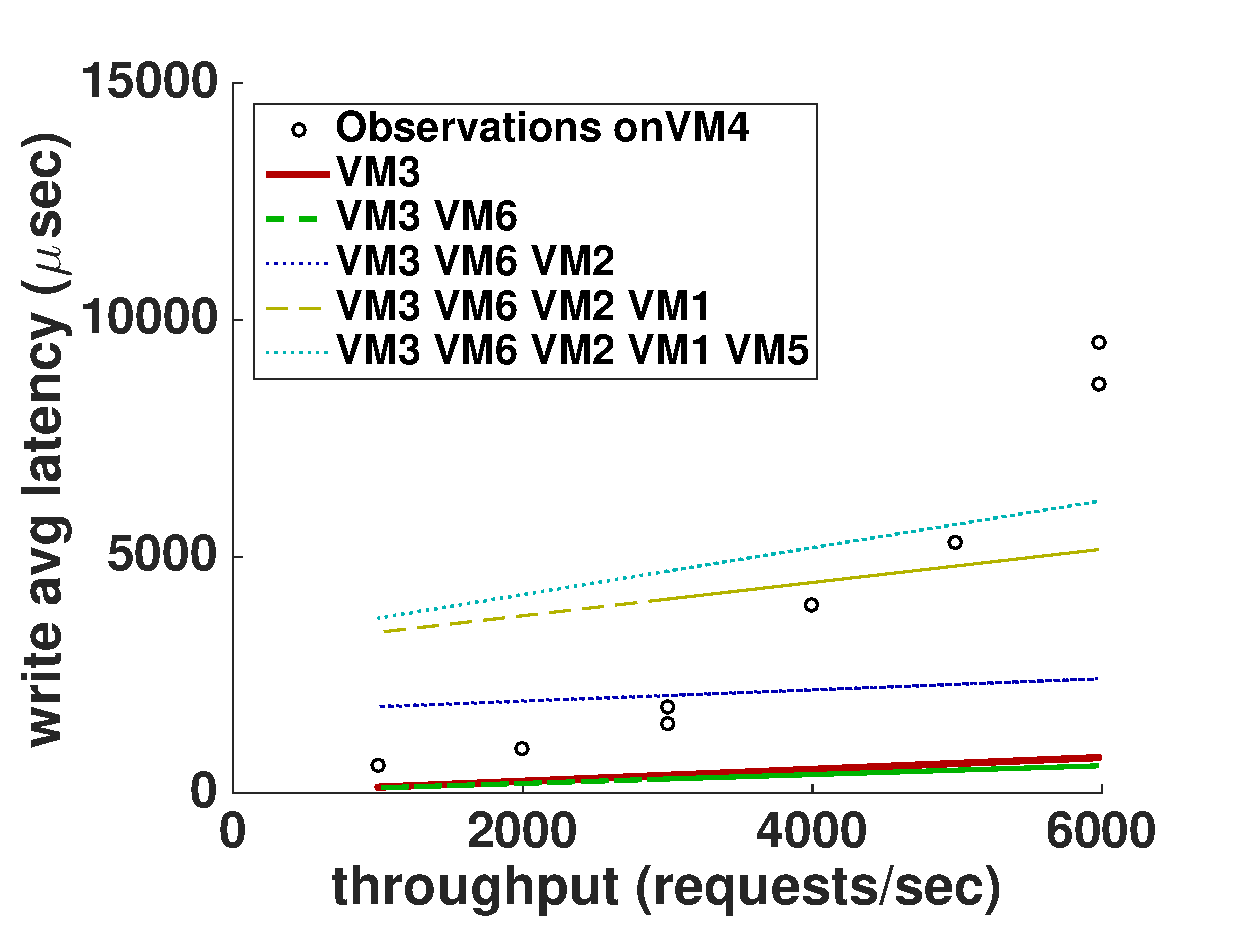
\includegraphics[width=0.5\textwidth]{cassandra_fit_write_avg_latency_m3_2x_r3_2x_m3_x_m3__r3_x_r3_.eps}}\\
\subfloat[fig 3]{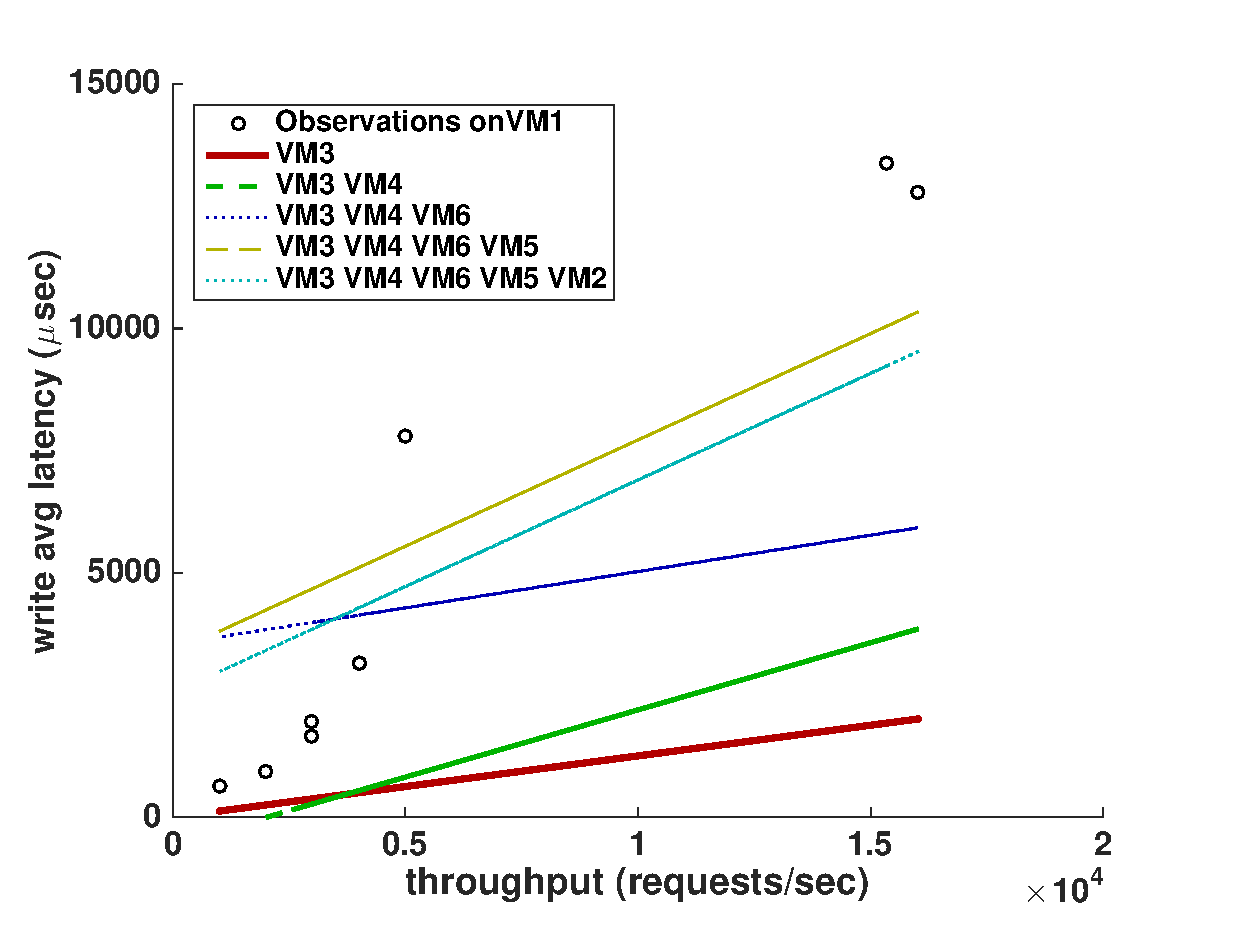
\includegraphics[width=0.5\textwidth]{cassandra_fit_write_avg_latency_m3_2x_r3__r3_2x_r3_x_m3_x_m3_.eps}}
\subfloat[fig 4]{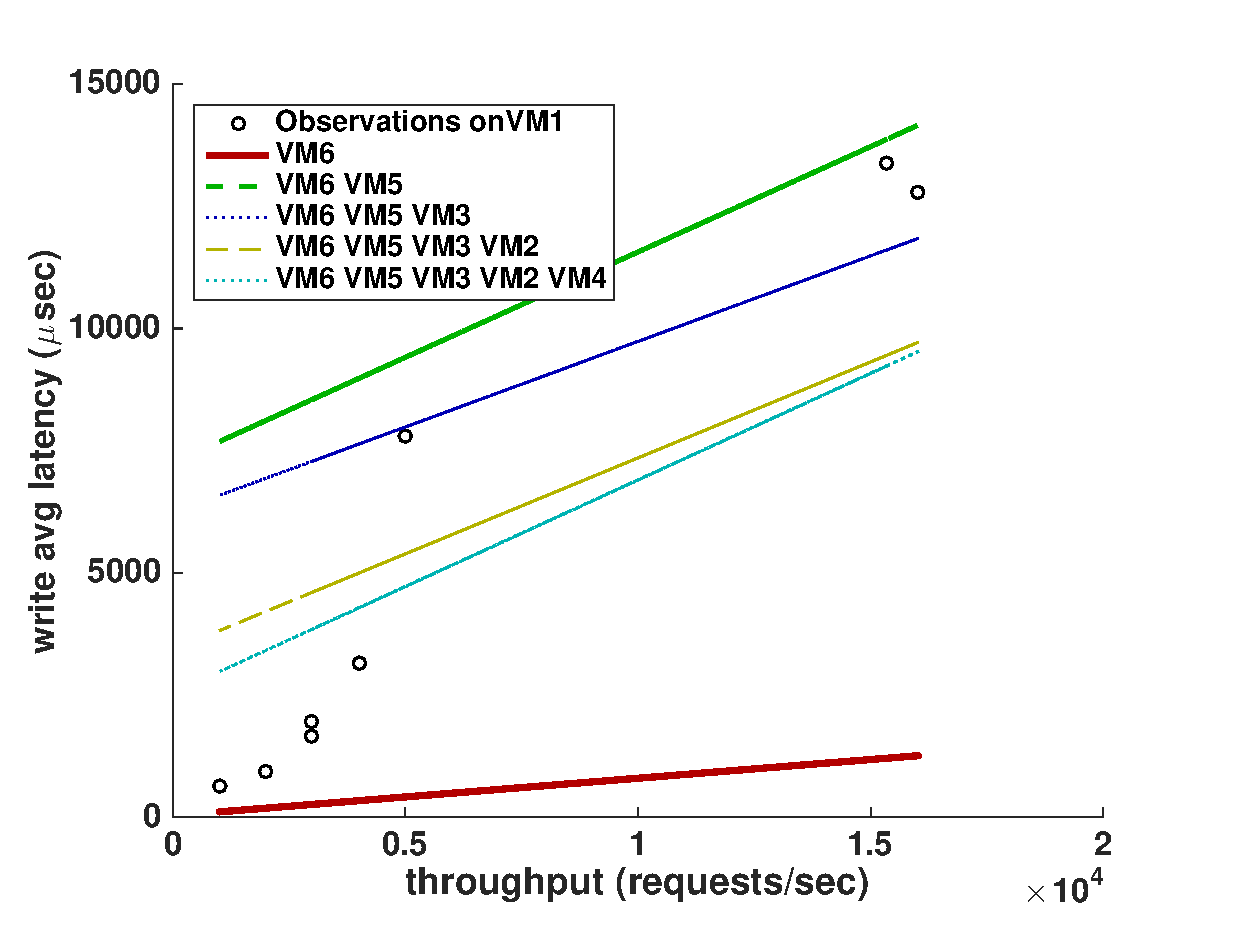
\includegraphics[width=0.5\textwidth]{cassandra_fit_write_avg_latency_r3_2x_r3_x_m3_2x_m3_x_r3__m3_.eps}} 
\caption{Incremental fit for Cassandra Average Write Latency }
\label{some example}
\end{figure*}

% \subsubsection{Evaluation for a Weak Consistency Configuration}

% consistency=ONE

% Workload B (95/5 r/w) with uniform distribution

% Present data for
% 3 VM types: gen,mem,cpu, throughputs 5000-20000, replication factor 3, 5 nodes

\subsection{MySQL}
\vspace{10pt}

\mm{
MySQL was deployed using Amazon Relational Database Service (Amazon RDS), which abstracts away the deployment and administration of OS and relationship database software.

MySQL was deployed to six VM types as listed in Table \ref{table:rdstypes}.

We tested using YCSB Workload A (50\% read, 50\% write) with a uniform distribution.

We did a multiple linear regression on the variables throughput, cores, memory, and network.  (Network performance was quantified by representing it as an dummy variable.)

We used VM type r3.2xlarge as test data, while increasing the training data in Table \ref{table:mysql}.

However, the data for MySQL did not fit a multilinear regression well.  This may be due to the higher write latency of SQL databases, or something with Amazon's RDS architecture that made our YCSB testing method unsuitable.  Another possibility is that the network availability varied over time with RDS, making data collection unrepeatable.
}

% \begin{table}
% \centering
% \caption{MySQL $R_{predicted}^2$ for $VM_6$}
% \begin{tabular}{|r|r|l|} \hline
% $R_{read}^2$&$R_{write}^2$&Training Data\\ \hline
% 0 & 0& $VM_1,VM_2,VM_3$\\ \hline
% 0 & 0& $VM_1,VM_2,VM_3,VM_4$\\ \hline
% 0 & 0& $VM_1,VM_2,VM_3,V_4,V_5$\\ \hline
% \hline\end{tabular}
% \label{table:mysql}
% \end{table}



